\documentclass[11pt]{article}

% ---------------------------------------------------------------- packages
\usepackage[utf8]{inputenc}
\usepackage[T1]{fontenc}
\usepackage{lmodern}
\usepackage[a4paper,margin=2.6cm]{geometry}
\usepackage{amsmath,amssymb,amsthm,mathtools}
\usepackage{booktabs,array,longtable}
\newcolumntype{P}[1]{>{\raggedright\arraybackslash}p{#1}}
\usepackage{slashed}
\usepackage{enumitem}
\usepackage{graphicx}
\usepackage{tikz}
\usetikzlibrary{positioning,arrows.meta}
\usepackage[numbers,sort&compress]{natbib}
\usepackage[colorlinks=true,linkcolor=blue!50!black,citecolor=blue!50!black,urlcolor=blue!50!black]{hyperref}
\usepackage{xcolor}
\usepackage[nameinlink,capitalise]{cleveref}

% ---------------------------------------------------------------- theorem styles
\theoremstyle{plain}
\newtheorem{theorem}{Theorem}[section]
\newtheorem{lemma}[theorem]{Lemma}
\newtheorem{proposition}[theorem]{Proposition}
\newtheorem{corollary}[theorem]{Corollary}
\theoremstyle{definition}
\newtheorem{definition}[theorem]{Definition}
\theoremstyle{remark}
\newtheorem{remark}[theorem]{Remark}
\newtheorem*{maintheorem*}{Main Theorem}

% ---------------------------------------------------------------- notation (defined where first used in the text)
\newcommand{\R}{\mathbb{R}}
\newcommand{\C}{\mathbb{C}}
\newcommand{\Q}{\mathbb{Q}}
\newcommand{\M}{\mathbb{M}}
\newcommand{\Dcal}{\mathcal{D}}
\newcommand{\Wcal}{\mathcal{W}}
\newcommand{\Ccal}{\mathcal{C}}
\newcommand{\rank}{\operatorname{rank}}
\newcommand{\xistar}{\xi^{*}}
\newcommand{\WP}{\mathrm{WP}}


\title{A Jordan-block obstruction to $L^2$ well-posedness\\ for charged spin-$3/2$ fields}
\pdftrailerid{}% reproducible build: no random PDF ID (with SOURCE_DATE_EPOCH set in build.sh)
\hypersetup{pdftitle={A Jordan-block obstruction to L2 well-posedness for charged spin-3/2 fields},pdfauthor={Sam DeRenzis}}
\author{Sam DeRenzis\\[2pt]
  \small \href{mailto:waitandhope123@gmail.com}{waitandhope123@gmail.com}\\
  \small Code and data: \href{https://doi.org/10.5281/zenodo.24413648}{doi:10.5281/zenodo.24413648}}
\date{\small Version 2, November 2026}

\begin{document}
\maketitle

\begin{abstract}
We study the Cauchy problem for a massive, charged Rarita--Schwinger (spin-$3/2$) field with a Pauli coupling, on the fixed background $\R_t\times S^2(1)\times S^2(3)$ threaded by a parallel magnetic field. The analysis is local, near one point. At one explicit parameter point we prove that no constants $K,\alpha$ exist for which existence, uniqueness and a loss-free $L^2$ energy bound all hold on small cones. The field equations are reduced exactly to an evolution equation for the spatial components, with a single constraint whose constrained subspace is preserved by the reduced operator. A constrained, variable-coefficient necessity lemma, whose hypotheses are verified here for this background, shows that such a package would force a resolvent bound for the principal symbol on the kernel of the constraint symbol. That bound is contradicted by an exact Jordan chain at a real eigenvalue, with entries in $\Q(i)$. The constraint for the time component is solvable, and every characteristic speed at the chosen covector is real. We do not identify which of the three properties fails, and we make no global or physical claim. The algebraic witness computations use exact arithmetic, and the scripts and data are publicly available.
\end{abstract}

\noindent\textbf{Keywords:} Rarita--Schwinger field; constrained hyperbolic systems; $L^2$ well-posedness; Jordan blocks; Velo--Zwanziger problem.\\
\textbf{MSC 2020:} 35L45, 35Q40, 81T20.

% =====================================================================
\section{Introduction}\label{sec:intro}

\subsection{The problem}\label{sec:intro-problem}

The Rarita--Schwinger equation \citep{RaritaSchwinger1941} describes a field of spin $3/2$. Coupling it consistently to other fields has been difficult from the start. Buchdahl studied the compatibility of the equations in a gravitational field \citep{Buchdahl1958}. For the charged field in an external electromagnetic field, Johnson and Sudarshan found that the equal-time quantisation relations of the local quantum theory are incompatible with relativistic covariance \citep{JohnsonSudarshan1961}. Velo and Zwanziger showed that the minimally coupled, charged field in an external electromagnetic potential propagates non-causally \citep{VeloZwanziger1969}. Inconsistencies in homogeneous magnetic fields were also found \citep{SeetharamanPrabhakaranMathews1975}. Many remedies and reformulations followed: modified wave equations \citep{Khalil1977}, supergravity \citep{DeserZumino1976}, and non-minimal couplings and their causality bounds \citep{DeserPascalutsaWaldron2000,DeserWaldron2002,PorratiRahman2009,Rahman2013}. Recent work revisits charged spin-$3/2$ fields in constant and Einstein--Maxwell backgrounds \citep{BenakliDanielKe2023,DelplanqueSkvortsov2024,Benakli2026,KrawczykEtAl2026}. The Velo--Zwanziger phenomenon itself has been revisited too \citep{Frauendiener2003}.

Much of this literature diagnoses problems through two tests: whether the constraint for the non-dynamical component can be solved, and whether the characteristic cones are real and causal. We ask a different, purely mathematical question, the standard one for hyperbolic systems: does the Cauchy problem admit a \emph{loss-free $L^2$ energy estimate}? For first-order systems, $L^2$ well-posedness is closely tied to the diagonalisability, or symmetrisability, of the principal symbol \citep{Kreiss1962,Strang1966,Strang1967,IvriiPetkov1974,Metivier2014,BenzoniGavageSerre2006,Rauch2012}. Systems whose principal symbol is not diagonalisable need separate treatment \citep{GarettoJahRuzhansky2018,ColombiniNishitaniRauch2019}. With constraints, the question is subtler \citep{AbalosReula2020,Abalos2022}, as numerical relativity has long known \citep{KreissOrtiz2002,NagyOrtizReula2004,SarbachTiglio2012}.

\subsection{Main result}\label{sec:intro-result}

We consider the field with a mass term and a Pauli coupling to a parallel magnetic field, on $\R_t\times S^2(1)\times S^2(3)$, near one point. At one explicit parameter point we prove the following (\cref{thm:main} gives the precise statement).

\begin{center}
\fbox{\parbox{0.9\linewidth}{\centering
\emph{There are no constants $K$ and $\alpha$ for which existence, uniqueness and the loss-free bound
$\|\Phi(t)\| \le Ke^{\alpha(t-s)}\|\Phi(s)\|$ all hold, for all constrained data, on any small cone around the base point, for any cone speed.}}}
\end{center}

\subsection{Mechanism}\label{sec:intro-mechanism}

The field equations reduce exactly to an evolution equation $\partial_t\Phi = K'\Phi$ for the spatial components, with one constraint $R^0\Phi = 0$, which $K'$ maps into itself in the sense $R^0K' = \Ccal R^0$ (\cref{sec:reduction}). At the witness point, the algebraic elimination matrix is invertible ($\det S^0 \neq 0$), and the reduced principal symbol has an entirely real spectrum at the selected nonzero covector $\xi^*$. This is a statement about one direction only: it does not establish real characteristics in every direction, or causality.
Yet $P(\xi^*)$ has a Jordan chain $v \to w$ at the real eigenvalue $r = 101/99$, and both vectors lie in the kernel of the constraint symbol $L(\xi^*)$. Everything here is exact, with entries in $\Q(i)$ (\cref{sec:witness}).

A necessity lemma (\cref{lem:necessity}) shows that the package would force the bound
\[
  \gamma|a| \le K_0\,|(\gamma - i(P - r))a| \qquad\text{for all } a \in \ker L,\ \gamma > 0 .
\]
Testing this on $a_\gamma = v - i\gamma w$ gives $|v| \le (1+K_0)\gamma|w|$. Letting $\gamma \to 0$ forces $v = 0$, which is a contradiction. \Cref{fig:chain} shows how the pieces fit together.

\begin{figure}[ht]
\centering
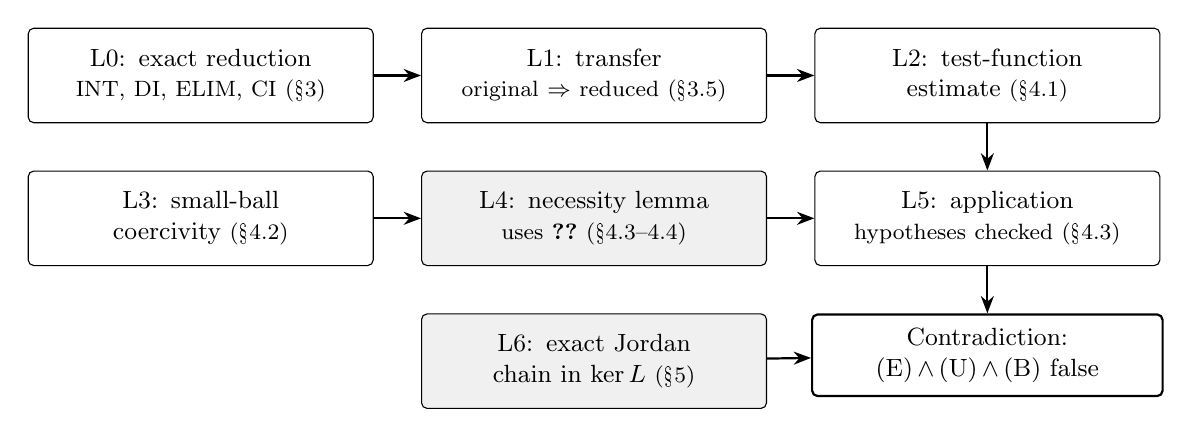
\begin{tikzpicture}[
  node distance=6mm and 6mm,
  box/.style={draw, rounded corners=2pt, align=center, font=\small, inner sep=4pt, minimum height=12mm, text width=41mm},
  key/.style={box, fill=black!6},
  arr/.style={-{Stealth[length=2.2mm]}, thick}]
\node[box] (L0) {L0: exact reduction\\ \footnotesize INT, DI, ELIM, CI\ (\S3)};
\node[box, right=of L0] (L1) {L1: transfer\\ \footnotesize original $\Rightarrow$ reduced (\S3.5)};
\node[box, right=of L1] (L2) {L2: test-function\\ estimate \footnotesize (\S4.1)};
\node[box, below=of L0] (L3) {L3: small-ball\\ coercivity \footnotesize (\S4.2)};
\node[key, below=of L1] (L4) {L4: necessity lemma\\ \footnotesize uses \cref{lem:osc} (\S4.3--4.4)};
\node[box, below=of L2] (L5) {L5: application\\ \footnotesize hypotheses checked (\S4.3)};
\node[key, below=of L4] (L6) {L6: exact Jordan\\ chain in $\ker L$ \footnotesize (\S5)};
\node[draw, thick, rounded corners=2pt, align=center, font=\small, inner sep=5pt, below=of L5, text width=41mm] (C) {Contradiction:\\ (E)$\,\wedge\,$(U)$\,\wedge\,$(B) false};
\draw[arr] (L0) -- (L1);
\draw[arr] (L1) -- (L2);
\draw[arr] (L2) -- (L5);
\draw[arr] (L3) -- (L4);
\draw[arr] (L4) -- (L5);
\draw[arr] (L5) -- (C);
\draw[arr] (L6) -- (C);
\end{tikzpicture}
\caption{Structure of the proof. Each box is one link of the proof chain. Arrows show which results each step uses. The shaded boxes are the two key ingredients: the necessity lemma, which turns an energy estimate into a resolvent bound on the constraint kernel, and the exact Jordan chain, which violates that bound. How each link was checked is summarised in \cref{tab:checking}.}
\label{fig:chain}
\end{figure}

\subsection{Relation to earlier work}\label{sec:intro-literature}

For first-order systems \emph{without} constraints, the fact that an $L^2$ estimate forces diagonalisability of the principal symbol goes back to Ivri\u{\i} and Petkov \citep{IvriiPetkov1974}. Métivier gave a wave-packet treatment with continuous coefficients \citep{Metivier2014}. Our \cref{lem:necessity} is a constrained, variable-coefficient analogue. Two features matter here. It only sees the kernel of the constraint symbol. And it does not assume that the principal symbol maps that kernel into itself.

Jordan blocks at real characteristic speeds are known in other higher-spin formulations. For example, a naive first-order form of minimal dRGT massive gravity is only weakly hyperbolic for this reason, and is reformulated by Ko\.zuszek and Wiseman \citep{KozuszekWiseman2024}. The defect found here sits on the principal symbol \emph{restricted to the exact constraint kernel} of the stated formulation, and it is transferred to the original field equations by \cref{lem:transfer}. For the massless field on vacuum curved spacetimes, Mason and Nicolas proved global existence and uniqueness for Rarita--Schwinger evolution equations compatible with the constraints \citep{MasonNicolas1999}. Their setting differs from ours (no mass, charge or Pauli term), and their result neither implies nor contradicts the present one. We have not completed a full comparison with the most recent work on charged spin-$3/2$ fields \citep{Benakli2026,KrawczykEtAl2026}, and we make no priority claim.

\subsection{What is and is not shown}\label{sec:intro-scope}

The theorem rules out the conjunction of existence, uniqueness and the loss-free bound for this local formulation. It does not say which property fails. It makes no claim about loss of derivatives, $C^\infty$ or Gevrey well-posedness, global questions, other formulations, or physics. \Cref{sec:scope} lists these limits and the open problems. The work was produced and checked by AI systems under the project owner's direction, and has not been reviewed by a human expert (\cref{app:checking}).

\subsection{Organisation}\label{sec:intro-organisation}

\Cref{sec:setting} fixes the setting and states the Main Theorem. \Cref{sec:reduction} carries out the exact reduction. \Cref{sec:analysis} proves the analytic ingredients and states the necessity lemma. \Cref{sec:witness} gives the witness and the proof. \Cref{sec:scope} discusses scope. The appendices contain the exact data and scripts (\cref{app:certificates}), the full proof of the necessity lemma (\cref{app:r1}), and an account of how the work was checked (\cref{app:checking}).

% =====================================================================
\section{Setting and statement}\label{sec:setting}

This section fixes the background, the equations and the parameters, defines the well-posedness package that is ruled out, and states the Main Theorem. Everything here is local: the analysis takes place in one coordinate chart around one base point.

\subsection{The background}\label{sec:background}

\paragraph{Spacetime and field strength.}
Let
\[
  \M = \R_t \times S^2(r_1) \times S^2(r_2), \qquad r_i = 1/b_i,\qquad b_1 = 1,\quad b_2 = \tfrac13 ,
\]
with the product of the flat time direction and the round metrics. On $\M$ we fix the magnetic field strength
\[
  F = b_1\, e^1\wedge e^2 + b_2\, e^3\wedge e^4 ,
\]
which is parallel, $\nabla F = 0$. The frame $e^A$ is defined below.

\paragraph{Chart, frame and volume.}
We work in coordinates $y = (\theta_1,\varphi_1,\theta_2,\varphi_2)$ on
\[
  V' = \bigl\{\, |\theta_i - \tfrac{\pi}{2}| < \tfrac{\pi}{3},\ |\varphi_i| < \tfrac{\pi}{3} \,\bigr\},
  \qquad y_0 = (\tfrac{\pi}{2},0,\tfrac{\pi}{2},0),
\]
on which $\sin\theta_i \ge \tfrac12$. The orthonormal frame is
\[
  e_0 = \partial_t,\quad
  e_1 = b_1\partial_{\theta_1},\quad
  e_2 = \frac{b_1}{\sin\theta_1}\partial_{\varphi_1},\quad
  e_3 = b_2\partial_{\theta_2},\quad
  e_4 = \frac{b_2}{\sin\theta_2}\partial_{\varphi_2},
\]
with dual coframe $e^A$. The Riemannian volume density is $\mu = \sin\theta_1\sin\theta_2/(b_1^2 b_2^2)$. Frame indices $A,B,\dots$ run over $0,\dots,4$, and spatial indices $a,j,k,\dots$ over $1,\dots,4$. The only non-zero connection coefficients $\nabla_{e_C}e_B = \omega^{A}{}_{B}(e_C)\,e_A$ are
\[
  \omega^{1}{}_{2}(e_2) = -\omega^{2}{}_{1}(e_2) = -b_1\cot\theta_1,\qquad
  \omega^{3}{}_{4}(e_4) = -\omega^{4}{}_{3}(e_4) = -b_2\cot\theta_2 .
\]
In particular nothing depends on $t$, and $\omega(e_0) = 0$.

\paragraph{Gauge potential.}
On $V'$ we use the local potential
\[
  A = -\cot\theta_1\, e^2 - \cot\theta_2\, e^4, \qquad dA = F .
\]
The field has non-zero flux through each sphere, so no global potential exists, and none is used.

\paragraph{Cones.}
Let $d$ be the Riemannian distance of the spatial metric. For $R, c > 0$ and $0 \le t < R/c$ set
\[
  B_t := \{\, y : d(y_0,y) < R - ct \,\}, \qquad
  \Ccal_s := \{\, (t,y) : s \le t \le T,\ y \in B_t \,\},
\]
with $L^2(B_t) := L^2(B_t, \mu\,dy;\C^{16})$ and the Euclidean norm on frame components. When we write $f \in C^j([s,T];X)$ on $\Ccal_s$, we mean that $f|_{[s,t_1]\times B_{t_1}} \in C^j([s,t_1];X(B_{t_1}))$ for every $t_1 \in [s,T]$. Likewise, an initial condition $\Phi(s) = \Phi_0$ means equality on every $B_{t_1}$.

\subsection{Field equations and the witness parameters}\label{sec:equations}

\paragraph{Clifford algebra.}
With $\eta = \operatorname{diag}(-1,1,1,1,1)$ we use the $4\times 4$ representation
\[
  \Gamma^0 = i\sigma_3\otimes 1,\quad
  \Gamma^1 = \sigma_1\otimes\sigma_1,\quad
  \Gamma^2 = \sigma_1\otimes\sigma_2,\quad
  \Gamma^3 = \sigma_1\otimes\sigma_3,\quad
  \Gamma^4 = \sigma_2\otimes 1,
\]
so that $\{\Gamma^A,\Gamma^B\} = 2\eta^{AB}$. Here $\Gamma^{ABC}$ denotes the unit-weight antisymmetrised product, equal to $\Gamma^A\Gamma^B\Gamma^C$ for distinct indices; $\Gamma_A = \eta_{AA}\Gamma^A$; and $\slashed{F} = F_{AB}\Gamma^A\Gamma^B$. Changing to an equivalent representation, or to the inequivalent one with $\Gamma^4 \to -\Gamma^4$, does not change the witness invariants used below (\cref{sec:robust}).

\paragraph{The field.}
The unknown is a vector-spinor $\psi = (\psi_0, \Phi)$ with frame components $\psi_A \in \C^4$. Its spatial part is $\Phi = (\psi_1,\dots,\psi_4) \in \C^{16}$.

\paragraph{Couplings and covariant derivative.}
Fix parameters $m > 0$, $\lambda \in \R$ and a charge $q \in \R$, and set $c_1 = i\sqrt{3/128}$. The mass and Pauli couplings are
\[
  X_A = -\frac{m}{3}\,\Gamma_A + \lambda c_1\Bigl(\slashed{F}\Gamma_A - \frac13\Gamma_A\slashed{F}\Bigr).
\]
With the spin connection $\Omega_C = \frac14\,\omega_{AB}(e_C)\,\Gamma^A\Gamma^B$ we define
\[
  (\nabla_B\psi)_C := e_B(\psi_C) - \omega^{A}{}_{C}(e_B)\,\psi_A + (\Omega_B + iqA_B)\,\psi_C,
  \qquad
  (\Dcal_B\psi)_C := (\nabla_B\psi)_C + X_B\,\psi_C .
\]

\paragraph{Equations.}
The field equations are
\begin{equation}\label{eq:RS}
  R^\rho[\psi] := \Gamma^{\rho\nu\sigma}\,(\Dcal_\nu\psi)_\sigma = 0, \qquad \rho = 0,\dots,4 .
\end{equation}
The $\rho = 0$ component, $R^0[\psi] = \Gamma^{0jk}(\Dcal_j\psi)_k$, contains no time derivative. It does not contain $\psi_0$ either, because $\Gamma^{00\sigma} = \Gamma^{0j0} = 0$ and $\omega^{0}{}_{k} = 0$. So $R^0$ is a first-order differential operator acting on $\Phi$ alone. The equation $R^0\Phi = 0$ is the \emph{constraint}.

\paragraph{The witness parameters.}
Throughout, the parameters are fixed at
\begin{equation}\label{eq:witness-params}
  \lambda^2 = \frac12,\qquad m^2 = \frac{823}{142944},\qquad q = \lambda\sqrt{\tfrac23}\,m ,
\end{equation}
together with the value $\pi' = \tfrac12$ of an auxiliary constraint-addition parameter that enters the reduction in \cref{sec:elim}. The relation $q = \lambda\sqrt{2/3}\,m$ defines what we call the \emph{Pauli slice}. At these values, the algebraic witness data used in \cref{sec:witness} are exact, with entries in $\Q(i)$. The sign of $\lambda$ does not matter: under $\lambda \to -\lambda$ the charge $q$ changes sign with it, and the matrices $S^\rho$, hence $\det S^0$, $P$, $L$ and the vectors $v,w$, are unchanged (checked exactly for both signs). The scripts use $\lambda = +1/\sqrt2$.

\subsection{The package that is ruled out}\label{sec:package}

\begin{definition}[Loss-free constrained $L^2$ package]\label{def:package}
Let $\ell \ge 2$ be an integer and $R, c, T > 0$. We say that $\WP^\ell(R,c,T)$ holds if there are constants $K \ge 1$ and $\alpha \ge 0$ such that, for every start time $s \in [0,T)$ and every $\Phi_0 \in H^\ell(B_s)$ with $R^0\Phi_0 = 0$ in $\mathcal{D}'(B_s)$, the following three properties hold.
\begin{description}
  \item[(E) Existence with regularity.] There is $\psi$ on $\Ccal_s$ with $\Phi \in C^1(H^{\ell-1}) \cap C(H^\ell)$ and $\psi_0 \in C(H^\ell)$, solving $R^\rho[\psi] = 0$ for $\rho = 0,\dots,4$, with $\Phi(s) = \Phi_0$.
  \item[(U) Uniqueness.] This $\psi$ is unique among all $\psi$ with $\Phi \in C^1(L^2)\cap C(H^1)$ and $\psi_0 \in C(H^1)$ that satisfy $R^\rho[\psi] = 0$ for all $\rho$ and $\Phi(s) = \Phi_0$.
  \item[(B) Loss-free $L^2$ bound.] For all $t \in [s,T]$,
  \[
    \|\Phi(t)\|_{L^2(B_t)} \le K\,e^{\alpha(t-s)}\,\|\Phi_0\|_{L^2(B_s)} .
  \]
\end{description}
\end{definition}

Property (B) is the standard energy-type estimate of $L^2$ well-posedness. It is \emph{loss-free} because the solution at time $t$ is controlled in the same norm as the data, with no loss of derivatives.

\subsection{Main Theorem}\label{sec:main-theorem}

\begin{theorem}[Main Theorem]\label{thm:main}
With the background of \cref{sec:background} and the parameters \eqref{eq:witness-params}, there is $r^* \in (0,\pi/6]$ such that, for every $R \in (0, r^*/2)$, every integer $\ell \ge 2$, every $c > 0$ and every $T \in (0, R/c)$, the package $\WP^\ell(R,c,T)$ is false.
\end{theorem}

In words: there are no constants $K$ and $\alpha$ for which existence, uniqueness and the loss-free $L^2$ bound all hold, for all start times and all constrained data, on any sufficiently small cone around $y_0$.

\begin{remark}[What the theorem says and does not say]\label{rem:scope}
\leavevmode
\begin{enumerate}
  \item The theorem rules out the \emph{conjunction} (E)\,$\wedge$\,(U)\,$\wedge$\,(B). It does not say which of the three properties fails.
  \item It holds for \emph{every} cone speed $c > 0$. So the failure cannot be repaired by taking wider cones.
  \item The radius $r^*$ comes from the coercivity estimate of \cref{sec:coer}. Its value plays no role beyond being positive.
  \item The statement concerns this local formulation. \Cref{sec:scope} lists what is not established.
\end{enumerate}
\end{remark}

% =====================================================================
\section{Exact reduction to a constrained evolution}\label{sec:reduction}

This section rewrites the field equations \eqref{eq:RS} exactly as an evolution equation for $\Phi$ alone, together with one constraint that the reduced operator maps into itself. No lower-order terms are dropped at any stage. The section ends with the transfer lemma, which carries the package of \cref{def:package} over to the reduced system.

\subsection{Clifford intertwining}\label{sec:int}

Alongside $X_A$ we use the \emph{adjoint coupling}
\[
  \hat Y_A = -\frac{m}{3}\,\Gamma_A + \lambda c_1\Bigl(\Gamma_A\slashed{F} - \frac13\slashed{F}\Gamma_A\Bigr),
\]
and the divergence of a vector-spinor field $V^A$,
\[
  (D+\hat Y)_A V^A := e_A(V^A) + \omega^{A}{}_{B}(e_A)\,V^B + (\Omega_A + iqA_A + \hat Y_A)\,V^A .
\]

\begin{lemma}[INT]\label{lem:int}
For all $\nu,\rho$, with summation over $\mu$: $\hat Y_\mu\Gamma^{\mu\nu\rho} = \Gamma^{\mu\nu\rho}X_\mu$.
\end{lemma}

\begin{proof}
The mass part is the standard contraction $\Gamma_\mu\Gamma^{\mu\nu\rho} = 3\Gamma^{\nu\rho} = \Gamma^{\mu\nu\rho}\Gamma_\mu$ in five dimensions. The $F$ part is linear in $F$. It is a finite identity, verified in exact arithmetic as a polynomial identity in $m$, $\lambda$ and the ten independent components of a general 2-form $F$ (script \texttt{check\_1}). A written Clifford-algebra proof of the $F$ part, in which the coefficient $\tfrac13$ is forced by the dimension being five, is recorded in the project archive. Here we rely on the exact computation.
\end{proof}

\subsection{The divergence identity}\label{sec:di}

\begin{proposition}[Divergence identity]\label{prop:di}
For every vector-spinor field $\psi$ (a distribution suffices),
\begin{equation}\label{eq:di}
  (D+\hat Y)_A\, R^A[\psi] = S^\rho\psi_\rho,
  \qquad
  S^\rho = \tfrac12 G^{\rho}{}_{\sigma}\Gamma^\sigma + \tfrac{iq}{2}\,\Gamma^{AB\rho}(dA)_{AB} + \Gamma^{AB\rho}(\nabla_AX)_B + \tfrac12\Gamma^{AB\rho}[X_A,X_B],
\end{equation}
where $G^{\rho}{}_{\sigma}$ is the Einstein tensor. Here, and throughout this proof, the contracted indices $A,B,C,D$ run over all five directions $0,\dots,4$; in particular the commutator sum includes the terms with $X_0$. On the background of \cref{sec:background}, the matrices $S^\rho$ are constant in the frame.
\end{proposition}

\begin{proof}
The argument works on any torsion-free spin 5-manifold.
\begin{enumerate}[label=(\roman*)]
  \item \emph{First derivatives cancel.} Put $W_{B\rho} := (\nabla\psi)_{B\rho} + X_B\psi_\rho$ and $V^A := \Gamma^{AB\rho}W_{B\rho}$. Since $\nabla\Gamma = 0$,
  \[
    \begin{aligned}(D+\hat Y)_AV^A = {}&\Gamma^{AB\rho}H_{AB}\psi_\rho + \Gamma^{AB\rho}(\nabla_AX_B)\psi_\rho + \Gamma^{AB\rho}X_B(\nabla\psi)_{A\rho}\\ &+ \hat Y_A\Gamma^{AB\rho}(\nabla\psi)_{B\rho} + \hat Y_A\Gamma^{AB\rho}X_B\psi_\rho ,\end{aligned}
  \]
  with $H_{AB} = \nabla_A\nabla_B - \nabla_{\nabla_Ae_B}$ the covariant Hessian. By \cref{lem:int} and the antisymmetry $\Gamma^{BA\rho} = -\Gamma^{AB\rho}$, the fourth term cancels the third. The fifth term equals $\tfrac12\Gamma^{AB\rho}[X_A,X_B]\psi_\rho$.
  \item \emph{Curvature.} By antisymmetry, $\Gamma^{AB\rho}H_{AB} = \tfrac12\Gamma^{AB\rho}(H_{AB} - H_{BA})$. Here $H_{AB} - H_{BA} = -R^{\sigma}{}_{\rho AB} + \Omega_{AB} + iq(dA)_{AB}$, where $\Omega_{AB} = \tfrac14 R_{CDAB}\Gamma^C\Gamma^D$. The first Bianchi identity removes the Riemann term acting on the vector index, and $\tfrac12\Gamma^{AB\rho}\Omega_{AB} = \tfrac12 G^{\rho}{}_{\sigma}\Gamma^\sigma$.
\end{enumerate}
The composite $(D+\hat Y)\circ R$ is a differential operator with smooth coefficients whose derivative terms all cancel, so \eqref{eq:di} also holds for distributions. Only on the background below do we specialise. There $\nabla X = 0$ because $\nabla F = 0$ and $\nabla\Gamma = 0$; $dA = F$; and
\[
  G^{\rho}{}_{\sigma} = \operatorname{diag}\bigl(-(b_1^2+b_2^2),\,-b_2^2,\,-b_2^2,\,-b_1^2,\,-b_1^2\bigr).
\]
So the $S^\rho$ are constant frame matrices. At the witness parameters they have entries in $\Q(i)$. The identity is also verified directly on the background by \texttt{check\_3}, for arbitrary component functions and symbolic $m,\lambda,b_1,b_2$.
\end{proof}

\subsection{Eliminating \texorpdfstring{$\psi_0$}{psi\_0}}\label{sec:elim}

As noted in \cref{sec:equations}, $R^0[\psi] = \Gamma^{0jk}(\Dcal_j\psi)_k$ contains neither $\partial_t$ nor $\psi_0$. For the spatial components we use $\omega(e_0) = 0$, $\Omega_0 = 0$ and $A_0 = 0$, which give $(\Dcal_0\psi)_k = \partial_t\psi_k + X_0\psi_k$. Since $\Gamma^{a00} = 0$,
\[
  R^a = -M^{ak}\,\partial_t\psi_k + Q^a[\psi],\qquad M^{ak} := \Gamma^{0ak},
\]
where $M = [M^{ak}]$ is an invertible $16\times16$ matrix and $Q^a$ contains only spatial derivatives (including those of $\psi_0$) and zeroth-order terms. In block notation write $R_{\mathrm{sp}} := (R^a)_{a=1}^4 \in \C^{16}$ and let $T\colon\C^4 \to \C^{16}$ be the constant block map $(T\rho)_a := \Gamma^0\Gamma^a\rho$. With the constraint-addition parameter $\pi'$, define
\[
  \tilde K(\Phi,\psi_0) := \partial_t\Phi + M^{-1}\bigl(R_{\mathrm{sp}} + \pi'\,TR^0\bigr),
\]
where $M^{-1}$ acts on the \emph{whole} bracket. This contains no time derivative; script \texttt{check\_4} confirms this. Since $(\partial_t - \tilde K)\Phi = -M^{-1}(R_{\mathrm{sp}} + \pi' TR^0)$, multiplying by $M$ gives, for arbitrary independent $\psi_0$ and $\Phi$,
\begin{equation}\label{eq:D}
  R_{\mathrm{sp}} = -M(\partial_t - \tilde K)\Phi - \pi'\,TR^0 .
\end{equation}
This is the convention implemented in the scripts, where the $\pi'$ term of the principal symbol also sits inside $M^{-1}$ (\cref{sec:symbols}).

\begin{lemma}[Elimination of $\psi_0$]\label{lem:elim}
At the witness parameters,
\[
  \det S^0 = \frac{3063716808343140625}{132101812606622109696} \neq 0 .
\]
Hence $S^\rho\psi_\rho = 0$ holds if and only if $\psi_0 = \Wcal\Phi$, where $\Wcal := -(S^0)^{-1}S^k$ (acting on $\Phi = (\psi_k)$) is a constant $4\times16$ frame matrix.
\end{lemma}

We define the reduced evolution operator
\[
  K'\Phi := \tilde K(\Phi,\,\Wcal\Phi).
\]
Besides $R^0\Phi = 0$, the reduction produces no further constraints. Its principal symbol is the matrix $P(y,k)$ of \cref{sec:symbols}.

\subsection{Constraint intertwining}\label{sec:ci}

\begin{lemma}[Contraction]\label{lem:contraction}
For a vector-spinor $h$ with $h_0 = 0$: $(D+\hat Y)_A\bigl(\Gamma^{A0C}h_C\bigr) = -R^0[h]$.
\end{lemma}

\begin{proof}
Let $n_B := \delta^0_B$; it is parallel. Put $V^A := \Gamma^{ABC}n_Bh_C$. Then $(\nabla V)^{A}{}_{A} = \Gamma^{ABC}n_B(\nabla_Ah)_C$, and by \cref{lem:int}, $\hat Y_AV^A = \Gamma^{ABC}X_An_Bh_C$. Adding the two gives
\[
  (D+\hat Y)_AV^A = \Gamma^{ABC}n_B(\Dcal_Ah)_C = \Gamma^{A0C}(\Dcal_Ah)_C = -\Gamma^{0AC}(\Dcal_Ah)_C = -R^0[h],
\]
using the sign convention $\Gamma^{A0C} = -\Gamma^{0AC}$.
\end{proof}

\begin{proposition}[Constraint intertwining]\label{prop:ci}
On the background, with $\psi_0 = \Wcal\Phi$,
\[
  R^0\,(\partial_t - K') = \star\, R^0,\qquad R^0K' = \Ccal\, R^0,
\]
as identities of differential operators acting on $\Phi$, where
\begin{align*}
  \star\rho &:= (\partial_t + \hat Y_0)\rho - \pi'\bigl[e_a(\Gamma^0\Gamma^a\rho) + \omega^{a}{}_{b}(e_a)\Gamma^0\Gamma^b\rho + (\Omega_a + iqA_a + \hat Y_a)\Gamma^0\Gamma^a\rho\bigr],\\
  \Ccal\rho &:= -\hat Y_0\rho + \pi'\bigl[e_a(\Gamma^0\Gamma^a\rho) + \omega^{a}{}_{b}(e_a)\Gamma^0\Gamma^b\rho + (\Omega_a + iqA_a + \hat Y_a)\Gamma^0\Gamma^a\rho\bigr].
\end{align*}
\end{proposition}

\begin{proof}
Split $R^A = R^0(e_0)^A + R^A_{\mathrm{sp}}$ with $R^A_{\mathrm{sp}} = (0,R^a)$. Since $e_0$ is parallel, $\Omega_0 = 0$ and $A_0 = 0$, we get $(D+\hat Y)_A\bigl(R^0(e_0)^A\bigr) = (\partial_t + \hat Y_0)R^0$. Insert \eqref{eq:D} into the divergence identity \eqref{eq:di}, and apply \cref{lem:contraction} to $h := (\partial_t - \tilde K)\Phi$, $h_0 := 0$. This gives, for arbitrary independent $\psi_0$ and $\Phi$,
\[
  R^0\bigl[(\partial_t - \tilde K)\Phi\bigr] = \star R^0\Phi - S^\rho\psi_\rho .
\]
This is an exact rearrangement of \eqref{eq:di}: no term is dropped, and no remainder arises. Script \texttt{check\_4} verifies it on the background for arbitrary $\psi_0$, $\Phi$ and symbolic $m,\lambda,b_1,b_2,\pi'$. Setting $\psi_0 = \Wcal\Phi$ removes $S^\rho\psi_\rho$ by \cref{lem:elim}, which gives the first identity. Since $R^0$ has time-independent coefficients, $R^0\partial_t = \partial_tR^0$, and the second identity follows.
\end{proof}

Both identities have smooth coefficients, so they hold on distributions. In particular, if $g \in H^{j+1}(B_s)$ and $R^0g = 0$, then $K'g \in H^j(B_s)$ and $R^0K'g = 0$. Only this algebraic mapping property is used below: for constrained $u$ the residual $f := (\partial_t - K')u$ again satisfies $R^0f = 0$, by the first identity. We do not need, and do not prove, that an arbitrary solution of $\partial_t\Phi = K'\Phi$ with $R^0\Phi(s) = 0$ stays constrained; that would require a uniqueness argument for $\partial_t\rho = \Ccal\rho$. The reduced package below already asks for constrained solutions.

\subsection{Transfer to the constrained evolution}\label{sec:transfer}

\begin{lemma}[Equivalence]\label{lem:equivalence}
On a fixed ball, let $\Phi \in C^1(L^2)\cap C(H^1)$ and $\psi_0 \in C(H^1)$. Then
\[
  R^\rho[\psi] = 0 \text{ for all } \rho
  \quad\Longleftrightarrow\quad
  \psi_0 = \Wcal\Phi,\quad \partial_t\Phi = K'\Phi,\quad R^0\Phi = 0 .
\]
\end{lemma}

\begin{proof}
($\Rightarrow$) Each $R^\rho$ lies in $C(L^2)$ and vanishes, so \eqref{eq:di} gives $S^\rho\psi_\rho = 0$ almost everywhere, and \cref{lem:elim} gives $\psi_0 = \Wcal\Phi$. Then \eqref{eq:D} gives $M(\partial_t - K')\Phi = -(R_{\mathrm{sp}} + \pi' TR^0) = 0$, and $R^0\Phi = 0$.
($\Leftarrow$) Put $\psi_0 = \Wcal\Phi$. Then $R^0 = 0$, and \eqref{eq:D} gives $R_{\mathrm{sp}} = 0$.
\end{proof}

Let $\WP_{\mathrm c}^\ell(R,c,T)$ denote the package for the reduced system. It consists of: (E$_{\mathrm c}$) a solution of $\partial_t\Phi = K'\Phi$ with $R^0\Phi = 0$, $\Phi \in C^1(H^{\ell-1})\cap C(H^\ell)$ and $\Phi(s) = \Phi_0$; (U$_{\mathrm c}$) uniqueness among constrained solutions in $C^1(L^2)\cap C(H^1)$; and (B$_{\mathrm c}$) the bound (B).

\begin{lemma}[Transfer]\label{lem:transfer}
If $\WP^\ell(R,c,T)$ holds with constants $K,\alpha$, then $\WP_{\mathrm c}^\ell(R,c,T)$ holds with the same $K$ and $\alpha$.
\end{lemma}

\begin{proof}
Existence and the bound follow from \cref{lem:equivalence} ($\Rightarrow$). For uniqueness, two constrained solutions $\Phi_1,\Phi_2$ give solutions $(\Wcal\Phi_i,\Phi_i)$ of the original equations in the class of (U), by \cref{lem:equivalence} ($\Leftarrow$). Here $\Wcal\Phi_i \in C(H^1)$ because $\Wcal$ is constant. So (U) forces $\Phi_1 = \Phi_2$.
\end{proof}

We write $U(t;s)\Phi_0$ for the solution given by (E$_{\mathrm c}$). By (U$_{\mathrm c}$), $U(t;s)$ is linear.

% =====================================================================
\section{Two analytic ingredients}\label{sec:analysis}

The proof combines the algebraic reduction of \cref{sec:reduction} with two analytic facts. The first, in \cref{sec:wh}, turns the package into an energy-type estimate that holds for every exactly constrained test function, not only for solutions. The second, in \cref{sec:coer}, is a coercivity estimate for the adjoint of the constraint on small balls. Together they supply the hypotheses of a necessity lemma (\cref{sec:r1}). That lemma converts the estimate into a bound on the principal symbol restricted to the constraint kernel. Its key analytic input is an oscillatory $H^{-1}$ bound (\cref{sec:osc}).

\subsection{From the package to an estimate on constrained test functions}\label{sec:wh}

Assume $\WP_{\mathrm c}^\ell(R,c,T)$ with constants $K,\alpha$, and let $U(t;s)$ be the solution operator of \cref{sec:transfer}.

\paragraph{Evaluation on full balls.}
Let $0 \le s \le s' < T$ and let $g \in H^\ell(B_s)$ be constrained. By the convention of \cref{sec:background} applied with $t_1 = s'$, we have $U(\cdot;s)g \in C([s,s'];H^\ell(B_{s'}))$. So $U(s';s)g$ lies in $H^\ell$ on the \emph{whole} ball $B_{s'}$, and it is constrained. It is therefore admissible data at start time $s'$. This is the only place where the convention matters, and it is used at every intermediate time below.

\begin{lemma}[Duhamel formula]\label{lem:duhamel}
Let $g \in H^{\ell+1}(B_s)$ be constrained, and let $r \in [s,T]$. Then, on $B_r$,
\[
  U(r;s)g = g + \int_s^r U(\sigma;s)K'g\,d\sigma ,
\]
a Bochner integral in $L^2(B_r)$.
\end{lemma}

\begin{proof}
By \cref{prop:ci}, $K'g \in H^\ell(B_s)$ is constrained. Put $v := U(\cdot;s)K'g$ and $w(t) := g + \int_s^t v$. Since $K'$ commutes with the integral, $K'w = K'g + v(t) - v(s) = v(t) = \partial_tw$. Moreover $w(s) = g$ and $R^0w = 0$. By (U$_{\mathrm c}$), $w = U(\cdot;s)g$.
\end{proof}

The semigroup property $U(t;s')U(s';s)g = U(t;s)g$ on $\Ccal_{s'}$ follows in the same way from (U$_{\mathrm c}$): both sides are constrained solutions with the same data at $s'$.

\begin{proposition}[Estimate on constrained test functions]\label{prop:wh}
Let
\[
  X^* := \bigl\{u \in C^1([0,T];H^\ell(B_0)) \cap C([0,T];H^{\ell+2}(B_0)) : R^0u(t) = 0 \text{ for all } t\bigr\}.
\]
Then for every $u \in X^*$ and $t \in [0,T)$,
\begin{equation}\label{eq:wh}
  \|u(t)\|_{L^2(B_t)} \le K e^{\alpha t}\|u(0)\|_{L^2(B_0)} + K\int_0^t e^{\alpha(t-\sigma)}\,\bigl\|(\partial_t - K')u(\sigma)\bigr\|_{L^2(B_\sigma)}\,d\sigma .
\end{equation}
\end{proposition}

\begin{proof}
Fix $t$ and $n$, and put $s_i = it/n$, $h = t/n$ and $B^{(i)} := B_{s_{i+1}}$.
\begin{enumerate}
  \item \emph{Telescoping.} Using $U(t;t) = \mathrm{id}$, the semigroup property and linearity, on $B_t$,
  \[
    u(t) - U(t;0)u(0) = \sum_i U(t;s_{i+1})\,d_i,
    \qquad d_i := u(s_{i+1})|_{B^{(i)}} - U(s_{i+1};s_i)u(s_i).
  \]
  Each $d_i$ lies in $H^\ell(B^{(i)})$ on the full ball, and it is constrained.
  \item \emph{Splitting $d_i$.} \Cref{lem:duhamel} with $g = u(s_i)$ gives
  \[
    d_i = \int_{s_i}^{s_{i+1}} (\partial_t - K')u\,d\sigma + e_i,
    \qquad
    e_i = \int_{s_i}^{s_{i+1}} \bigl[K'u(\sigma) - U(\sigma;s_i)K'u(s_i)\bigr]\,d\sigma .
  \]
  \item \emph{The error terms.} The time variation of $K'u$ costs at most
  $Ch\sup_\tau\|\partial_tu(\tau)\|_{H^1}$. Applying \cref{lem:duhamel} to the constrained datum $K'u(s_i)$, together with the bound (B$_{\mathrm c}$) for $(K')^2u(s_i)$, which is constrained by \cref{prop:ci}, gives $\|U(\sigma;s_i)K'u(s_i) - K'u(s_i)\| \le hKe^{\alpha T}\|(K')^2u(s_i)\|$. Hence $\|e_i\|_{L^2(B^{(i)})} \le C_u h^2$.
  \item \emph{Summing.} Apply (B$_{\mathrm c}$) to each $d_i$, and use $e^{\alpha(t - s_{i+1})} \le e^{\alpha(t-\sigma)}$ for $\sigma \le s_{i+1}$. The terms $e_i$ contribute at most $KC_ue^{\alpha T}t^2/n$, which tends to $0$ as $n \to \infty$.
\end{enumerate}
The evolution is applied only to constrained data, never to the residual $(\partial_t - K')u$.
\end{proof}

\subsection{Small-ball coercivity}\label{sec:coer}

In the chart, $R^0\Phi = \sum_j L_j(y)\partial_j\Phi + L_0(y)\Phi$, with $L_j(y) = \sum_a E_a^{\,j}(y)\,[\Gamma^{0ak}]_k$ and $L_0$ smooth on $\overline{V'}$. Its formal adjoint with respect to $\mu\,dy$ is
\[
  R^{0*}\rho = -\sum_j L_j^\dagger\partial_j\rho + M_0\rho,
  \qquad
  M_0 := L_0^\dagger - \sum_j \mu^{-1}\partial_j\bigl(\mu L_j^\dagger\bigr).
\]

\begin{proposition}[Small-ball coercivity]\label{prop:coer}
There are $r_0 > 0$ and $c_0 > 0$ such that, for every $\rho' \le \pi/6$ with $2\rho' \le r_0$, the geodesic ball $B' := B_d(y_0,\rho')$ satisfies
\begin{equation}\label{eq:coer}
  \|R^{0*}\rho\|_{L^2(B',\mu)} \;\ge\; c_0\,\|\rho\|_{H^1}
  \qquad\text{for all } \rho \in H^1_0(B') .
\end{equation}
\end{proposition}

\begin{proof}
\begin{enumerate}[label=(\alph*)]
  \item \emph{Symbol bound.} In the frame, $L(\xi)L(\xi)^\dagger = 3|\xi|^2I_4$ for all $\xi$. This identity is exact; it is checked by \path{witness_min.py} and \path{check_2}. In the chart, $L(y,k) = L(\xi)$ with
  \[\xi = (b_1k_1,\ b_1k_2/\sin\theta_1,\ b_2k_3,\ b_2k_4/\sin\theta_2),\]
  so $|\xi| \ge \underline\beta\,|k|$ with $\underline\beta := \min(b_1,b_2) = \tfrac13$. Hence $|L(y,k)^\dagger v| \ge \sigma|k||v|$ with $\sigma := \sqrt3\,\underline\beta$.
  \item \emph{Frozen coefficients.} On a Euclidean chart ball $\mathcal U_r = B_e(y_0,r)$ with $r \le \pi/3$, Plancherel gives $\|\sum_j L_j(y_0)^\dagger\partial_j\rho\|_{L^2(dy)} \ge \sigma\|\nabla\rho\|$ for $\rho \in C^\infty_c(\mathcal U_r)$.
  \item \emph{Freezing error.} Only $E_2$ and $E_4$ vary, and $|\partial_\theta(1/\sin\theta)| \le 2\sqrt3$ on $V'$. Each row of $[\Gamma^{0ak}]_k$ has three unitary blocks. This gives $\bigl(\sum_j\|L_j(y) - L_j(y_0)\|^2\bigr)^{1/2} \le \ell_1 r$ on $\mathcal U_r$, with $\ell_1 := 6\sqrt{b_1^2 + b_2^2}$.
  \item \emph{Lower-order term.} $m_0 := \sup_{\overline{V'}}\|M_0\| < \infty$, because all coefficients are smooth on $\overline{V'}$. Its value is not needed. The Poincaré inequality on a ball of radius $r$ in $\R^4$ gives $\|\rho\| \le r\|\nabla\rho\|$, since the first Dirichlet eigenvalue is $(j_{1,1}/r)^2$ and $j_{1,1} > 1$.
  \item \emph{Absorption.} Combining (b)--(d), $\|R^{0*}\rho\|_{L^2(dy)} \ge (\sigma - (\ell_1 + m_0)r)\|\nabla\rho\|$. With $\inf_{V'}\mu \ge 1/(4b_1^2b_2^2)$ and $\|\rho\|_{H^1}^2 \le (1+r^2)\|\nabla\rho\|^2$, this yields \eqref{eq:coer} on $\mathcal U_r$ for
  \[ r \le r_0 := \min\bigl(\pi/3,\ \sigma/(2(\ell_1 + m_0))\bigr). \]
  \item \emph{Geodesic balls.} On $V'$ the chart metric is at least $\tfrac14 I$. So for $\rho' \le \pi/6$ we have $B_d(y_0,\rho') \subset B_e(y_0,2\rho') \subset V'$. Extension by zero embeds $H^1_0$ of the first ball into $H^1_0$ of the second.
\end{enumerate}
\end{proof}

We fix $r^* := \min(\pi/6,\ r_0/2)$; this is the radius in \cref{thm:main}. We use the balls
\[
  B' := B_d(y_0,r^*),\qquad B'' := B_d(y_0,3r^*/4),\qquad B := B_d(y_0,R),\quad R < r^*/2 ,
\]
so that $B \Subset B'' \Subset B'$ and \eqref{eq:coer} holds on $B'$.

\subsection{The necessity lemma}\label{sec:r1}

We state the lemma in the generality in which it is proved. Let $B \Subset B'' \Subset B' \subset \R^4$ be bounded open sets, $T > 0$, and $\{B_t\}_{t\in[0,T]}$ a family of open sets. Let $K = \sum_j A_j\partial_j + \mathfrak{B}$ ($n\times n$) and $R = \sum_j L_j\partial_j + L_0$ ($n'\times n$) be time-independent operators, with symbols $P(y,k) = \sum_j k_jA_j(y)$ and $L(y,k) = \sum_j k_jL_j(y)$. Let $\mu$ be a positive weight function; all $L^2$ norms below use the measure $\mu\,dy$. Let $s \ge 2$ be an integer. The hypotheses are:
\begin{description}
  \item[(Pos)] $0 < \inf_{B'}\mu \le \sup_{B'}\mu < \infty$.
  \item[(Reg$_s$)] $\mu, L_j \in C^{s,1}(\overline{B'})$, $L_0 \in C^{s-1,1}(\overline{B'})$, $A_j \in C^{0,1}(\overline B)$ and $\mathfrak B \in L^\infty(B)$.
  \item[(C1)] $\|R^*\rho\|_{L^2(B',\,\mu\,dy)} \ge c_0\|\rho\|_{H^1}$ for all $\rho \in H^1_0(B')$, where $R^*$ is the formal adjoint with respect to $\mu\,dy$.
  \item[(BT)] $B_0 = B$, and the $B_t$ decrease. For the point $y_1$ in question there are $t_0 \in (0,T)$ and $\varepsilon > 0$ with $\overline{B(y_1,\varepsilon)} \subset B_{t_0}$.
  \item[(H$_X$)] There are $K_0 \ge 1$ and $\alpha \ge 0$ such that the estimate \eqref{eq:wh}, with $K_0$ in place of $K$ and norms taken with respect to $\mu\,dy$, holds for every $u$ in a class $X \subset C^1([0,T];L^2(B))\cap C([0,T];H^s(B))$ of functions with $Ru(t) = 0$. The class must contain the wave packets constructed in the proof.
\end{description}

\begin{theorem}[Necessity lemma]\label{lem:necessity}
Under these hypotheses,
\[
  \gamma\,|a| \;\le\; K_0\,\bigl|\bigl(\gamma - i(P(y_1,k) - \tau)\bigr)a\bigr|
\]
for all $k \neq 0$, $\tau \in \R$, $\gamma > 0$ and $a \in \ker L(y_1,k)$.
\end{theorem}

The lemma does \emph{not} assume that $P$ maps $\ker L$ into itself. It is a constrained, variable-coefficient analogue of the necessity direction in the work of Ivri\u{\i} and Petkov \citep{IvriiPetkov1974} and of Métivier \citep{Metivier2014}. The complete proof is in \cref{app:r1}. Its four steps are as follows.
\begin{enumerate}
  \item \emph{Packet.} Take a spatial wave packet $q_\Lambda = e^{i\Lambda k\cdot(y-y_1)}\chi_\kappa\,a$, with amplitude $a \in \ker L(y_1,k)$ and a bump $\chi_\kappa$ of width $\kappa = \Lambda^{-1/2}$ around $y_1$.
  \item \emph{Exact constraint.} Subtract the correction $W_\Lambda := R^*\mathcal{G}(Rq_\Lambda)$. Here $\mathcal G$ solves the Dirichlet problem for $RR^*$ on $B'$ by Lax--Milgram, using (C1). The corrected packet $p_\Lambda := q_\Lambda - W_\Lambda$ satisfies $Rp_\Lambda = 0$ exactly, and interior elliptic regularity shows that $u_\Lambda(t) := e^{\Lambda(\gamma+i\tau)t}p_\Lambda$ is admissible.
  \item \emph{Small correction.} The correction is small, $\|W_\Lambda\| = O(\Lambda^{-1/2})\|q_\Lambda\|$, because the constraint residual $Rq_\Lambda$ oscillates at frequency $\Lambda$. This is where \cref{lem:osc} enters.
  \item \emph{Single-time limit.} Apply (H$_X$) to $u_\Lambda$ at the time $t_0$. The main term of $(\partial_t - K)u_\Lambda$ is $\Lambda e^{i\theta}\chi_\kappa\bigl(\gamma - i(P(y_1,k) - \tau)\bigr)a$, and the rest is $O(\Lambda^{1/2})$. Dividing by $e^{\Lambda\gamma t_0}\|q_\Lambda\|$ and letting $\Lambda \to \infty$ at fixed $\gamma$ gives the bound with the same constant $K_0$.
\end{enumerate}

\paragraph{Application to our system.}
We apply \cref{lem:necessity} with $K = K'$, $R = R^0$, $n = 16$, $n' = 4$, the weight $\mu$ (the volume density of \cref{sec:background}), the balls of \cref{sec:coer}, and $B_t$ the cone balls of \cref{sec:background}.
\begin{itemize}
  \item (Pos) and (Reg$_s$) hold for every $s$: all coefficients are smooth on $\overline{V'}$, where $\sin\theta_i \ge \tfrac12$.
  \item (C1) is \cref{prop:coer}.
  \item The ball conditions hold. The $B_t$ are open and decreasing. Every $y_1 \in B$ satisfies the interior condition: choose $t_0 > 0$ so small that $y_1 \in B_{t_0}$, and use the continuity of $d$ and the chart bound $d(y,y_1) \le 3|y - y_1|$.
  \item (H$_X$) holds on $X = X^*$ with $K_0 = K$, by \cref{prop:wh}. The functions $u_\Lambda$ lie in $X^*$. The coefficients are smooth, so interior regularity of every order (\cref{lem:hs} with $s = \ell + 2$) gives $p_\Lambda \in H^{\ell+2}(B)$. Moreover $p_\Lambda$ is constrained, and the time factor is smooth.
\end{itemize}

\subsection{The oscillatory \texorpdfstring{$H^{-1}$}{H\^{}-1} bound}\label{sec:osc}

The step that makes the correction $q_\Lambda$ negligible is the following estimate. Here $H^{-1}_\mu(B')$ is the dual of $H^1_0(B')$ under the pairing weighted by $\mu$.

\begin{lemma}[Oscillatory $H^{-1}$ bound]\label{lem:osc}
For $g \in H^2$ with compact support in $B'$, $\Lambda > 0$ and $k \neq 0$,
\[
  \|e^{i\Lambda k\cdot y}g\|_{H^{-1}_\mu}
  \;\le\; C_\mu\Bigl(\frac{2}{\Lambda|k|}\,\|g\|_{L^2} + \frac{4}{(\Lambda|k|)^2}\,\|D^2g\|_{L^2}\Bigr),
  \qquad C_\mu := \|\mu\|_\infty + \|\nabla\mu\|_\infty .
\]
\end{lemma}

\begin{proof}
Without the weight,
\[
  \|e^{i\Lambda k\cdot y}g\|_{H^{-1}}^2 = \int \langle\eta + \Lambda k\rangle^{-2}|\hat g(\eta)|^2\,d\eta .
\] Split at $|\eta| = \Lambda|k|/2$. For $|\eta| \le \Lambda|k|/2$ we have $\langle\eta + \Lambda k\rangle \ge \Lambda|k|/2$, so this region contributes at most $(2/(\Lambda|k|))^2\|g\|^2$. For $|\eta| > \Lambda|k|/2$ we use $\langle\cdot\rangle^{-2} \le 1$ and $1 \le (2|\eta|/(\Lambda|k|))^4$, together with the exact identity $\int|\eta|^4|\hat g|^2 = \|D^2g\|^2$ (valid for compact support). This region contributes at most $(2/(\Lambda|k|))^4\|D^2g\|^2$. Taking square roots, and moving the weight onto the test function, which costs the factor $C_\mu$, completes the proof.
\end{proof}

\begin{remark}[Why two derivatives]\label{rem:two-derivatives}
The second derivatives are essential to the argument.
\begin{itemize}
  \item A bound of the form $\|e^{i\Lambda k\cdot y}g\|_{H^{-1}} \le C\Lambda^{-1}\|g\|_{L^2}$ for arbitrary $g \in L^2$ is \emph{false}. Take $g = e^{-i\Lambda k\cdot y}g_0$ with a fixed $0 \neq g_0 \in C^\infty_c$: the left side stays fixed while the right side tends to zero.
  \item A bound with one derivative of $g$ holds, but it is too weak for the amplitudes that occur in the packet construction.
\end{itemize}
The two-derivative bound is what makes the correction of the packet negligible in \cref{app:r1-sizes}.
\end{remark}

% =====================================================================
\section{The witness and the contradiction}\label{sec:witness}

This section exhibits an explicit, exact Jordan chain of the principal symbol inside the kernel of the constraint symbol, and uses it to prove \cref{thm:main}. Everything in \cref{sec:symbols,sec:chain} is exact rational arithmetic over $\Q(i)$. The data are listed in \cref{app:certificates}.

\subsection{Symbols at the base point}\label{sec:symbols}

The reduction of \cref{sec:reduction} turns the field equations into an evolution equation $\partial_t\Phi = K'\Phi$ for $\Phi$ alone, together with the constraint $R^0\Phi = 0$. In the chart we write the first-order parts as
\[
  K'\Phi = \sum_{j} K_j(y)\,\partial_j\Phi + (\text{zeroth order}),\qquad
  R^0\Phi = \sum_{j} L_j(y)\,\partial_j\Phi + L_0(y)\Phi ,
\]
and define the principal symbols, for a covector $k \in \R^4$,
\[
  P(y,k) := \sum_j k_j K_j(y) \quad (16\times 16), \qquad
  L(y,k) := \sum_j k_j L_j(y) \quad (4\times 16).
\]
So the symbol of $K'$ is $iP(y,k)$. Both symbols are frame expressions evaluated at $\xi = E(y)^{T}k$, where $E(y)$ is the diagonal matrix of frame components from \cref{sec:background}, that is $\xi = (b_1k_1,\ b_1k_2/\sin\theta_1,\ b_2k_3,\ b_2k_4/\sin\theta_2)$. Explicitly,
\[
  L(\xi) = \Bigl[\ \textstyle\sum_j \xi_j\,\Gamma^{0jk}\ \Bigr]_{k},\qquad
  P(\xi) = M^{-1}\Bigl[\ \textstyle\sum_j \xi_j\bigl(\Gamma^{ijk} - \Gamma^{0ij}(S^0)^{-1}S^k + \pi'\,\Gamma^0\Gamma^i\Gamma^{0jk}\bigr)\Bigr]_{ik},
\]
with $M := [\Gamma^{0ik}]_{ik}$ and the constant frame matrices $S^\rho$ of the divergence identity (\cref{sec:di}). The formula for $P$ is derived from the principal parts in \cref{sec:reduction}. It is also checked directly on the curved operator at $y_0$ (script \texttt{check\_5}, \cref{app:certificates}).

At the base point $y_0$ we choose
\[
  k^* = \bigl(\tfrac{20}{99},\,0,\,3,\,0\bigr), \qquad\text{so that}\qquad
  \xi^* = E(y_0)^{T}k^* = \bigl(\tfrac{20}{99},\,0,\,1,\,0\bigr),
\]
and write $P := P(y_0,k^*) = P(\xi^*)$ and $L := L(y_0,k^*) = L(\xi^*)$. \Cref{tab:jordan} collects their exact properties.

\begin{table}[ht]
\centering
\caption{Exact algebraic data at the witness. All entries were computed in exact arithmetic over $\Q(i)$. They are reproduced by the scripts in \cref{app:certificates} and by the validator's checks D1--D3.}
\label{tab:jordan}
\renewcommand{\arraystretch}{1.25}
\begin{tabular}{@{}P{4.2cm} P{10.4cm}@{}}
\toprule
Quantity & Exact value \\
\midrule
$\det S^0$ & $3063716808343140625 \,/\, 132101812606622109696 \;\neq 0$ \\
Spectrum of $P(\xi^*)$ (at $\pi' = \tfrac12$) & $\pm\tfrac{101}{99}$, each of algebraic multiplicity 6, and $\pm\tfrac{101}{198}$, each of multiplicity 2. All real. \\
Chosen eigenvalue & $r = \tfrac{101}{99}$\quad (note $r = |\xi^*|$) \\
$\dim\ker(P - r)^j$, $j = 1,2,3$ & $4,\ 6,\ 6$\quad (two Jordan blocks of size 2, two of size 1) \\
$\rank L(\xi^*)$ & $4$, so $\dim\ker L(\xi^*) = 12$ \\
Constraint symbol & $L(\xi)L(\xi)^\dagger = 3|\xi|^2 I_4$ for all $\xi$ \\
\bottomrule
\end{tabular}
\end{table}

The constraint kernel is an invariant subspace of $P$, and $P$ induces a map on the quotient; the quotient part of the spectrum is set by the constraint addition.

\begin{proposition}[Structure of the symbol]\label{prop:structure}
Write $P_{\pi'}$ for the symbol with constraint-addition parameter $\pi'$, and $C_1(\xi) := \pi'\sum_a\xi_a\Gamma^0\Gamma^a$ $(4\times4)$.
\begin{enumerate}[label=(\alph*)]
  \item $P_{\pi'}(\xi) - P_{\pi''}(\xi) = (\pi' - \pi'')\,M^{-1}T\,L(\xi)$ for all $\xi$. In particular $P_{\pi'}$ restricted to $\ker L(\xi)$ does not depend on $\pi'$.
  \item $L(\xi)P_{\pi'}(\xi) = C_1(\xi)L(\xi)$ for all $\xi$. Hence $P_{\pi'}(\xi)\ker L(\xi) \subseteq \ker L(\xi)$.
  \item At $\xi^*$, for every $\pi'$, the characteristic polynomial of $P_{\pi'}$ is $(x^2 - r^2)^6\,(x^2 - \pi'^2r^2)^2$.
\end{enumerate}
\end{proposition}

\begin{proof}
(a) The only $\pi'$-dependent term in the formula for $P$ is $\pi'M^{-1}[\sum_j\xi_j\Gamma^0\Gamma^i\Gamma^{0jk}]_{ik} = \pi'M^{-1}T\,L(\xi)$. (b) Taking principal symbols of the second-order identity $R^0K' = \Ccal R^0$ of \cref{prop:ci}: the symbol of $R^0$ is $iL$, that of $K'$ is $iP$, and the first-order symbol of $\Ccal$ is $iC_1$, which gives $LP = C_1L$. (c) By (b), $P$ acts on the quotient $\C^{16}/\ker L \cong \C^4$ as $C_1$. Write $\Gamma(\xi) := \sum_a\xi_a\Gamma^a$, so $C_1 = \pi'\Gamma^0\Gamma(\xi)$. Since $\Gamma^0$ anticommutes with each $\Gamma^a$ and $(\Gamma^0)^2 = -I$, we get $\Gamma^0\Gamma(\xi)\Gamma^0 = \Gamma(\xi)$; and $\Gamma(\xi)^2 = |\xi|^2I$. Hence $C_1(\xi)^2 = \pi'^2\Gamma(\xi)^2 = \pi'^2|\xi|^2I$. For $\xi \neq 0$ and $\pi' \neq 0$, $C_1$ is traceless with $C_1^2 = \pi'^2|\xi|^2I$, so the quotient has eigenvalues $\pm\pi'|\xi|$, each of multiplicity two; at $\xi^*$ these are $\pm\pi' r$. At $\pi' = 0$, $C_1 = 0$ and the quotient has the single eigenvalue $0$ with multiplicity four. The formula below covers both cases. By (a), the restriction to the 12-dimensional $\ker L$ is the one at $\pi' = \tfrac12$, whose eigenvalues are $\pm r$, each six times. Parts (a)--(c) were also checked in exact arithmetic with $\pi'$ symbolic; checks of (b) and of $C_1^2 = \pi'^2|\xi|^2I$ at random rational covectors are regression tests only.
\end{proof}

So the eigenvalues $\pm\tfrac{101}{198}$ in \cref{tab:jordan} are $\pm\pi'|\xi^*|$ at $\pi' = \tfrac12$ and are eigenvalues of the induced map on the quotient. This is an invariant subspace and a quotient, not an invariant direct-sum decomposition. At $\pi' = \pm1$ the quotient and constrained eigenvalues coincide, and the characteristic polynomial alone does not determine the full Jordan structure of $P$ on $\C^{16}$ there. The witness does not depend on this: the chain $v \to w$ lies in $\ker L$, and by part (a) it is the same for every $\pi'$. This answers the question whether the chain could be an artefact of the choice $\pi' = \tfrac12$, but only for this one-parameter family of constraint additions; it says nothing about other formulations. Although \cref{lem:necessity} does not require invariance of $\ker L$, part (b) shows that it holds for the present system.

The eigenvalues are given at the non-unit covector $\xi^*$, with $|\xi^*| = \tfrac{101}{99}$. Relative to the unit covector $\xi^*/|\xi^*|$ they become $\pm1$ and $\pm\pi' = \pm\tfrac12$. These are directional speeds in this one direction only. Nothing here is a statement about all directions or about causality.

\subsection{The Jordan chain}\label{sec:chain}

\begin{proposition}[Exact witness chain]\label{prop:chain}
Let $r = 101/99$, and let $v, w \in \Q(i)^{16}$ be the vectors listed in \cref{app:certificates}. Then
\[
  Lv = 0,\qquad Lw = 0,\qquad (P - r)\,v = 0,\qquad (P - r)\,w = v,\qquad v \neq 0 .
\]
By \cref{prop:structure}(a), the same relations hold for every value of $\pi'$.
\end{proposition}

\begin{proof}
This is a finite computation in exact rational arithmetic over $\Q(i)$, carried out by the script \texttt{witness\_min.py}. It is reproduced separately by \texttt{data/read\_witness.py}, which uses only Python's built-in fractions, and by the validator's check D1 (\cref{app:certificates}). All three are code from this project, so this is a cross-check, not independent replication.
\end{proof}

So $v \to w$ is a Jordan chain of length two for $P$ at the real eigenvalue $r$, and both vectors satisfy the linearised constraint. That combination is what the necessity lemma rules out.

\subsection{Proof of the Main Theorem}\label{sec:proof}

\begin{proof}[Proof of \cref{thm:main}]
Suppose, for contradiction, that $\WP^\ell(R,c,T)$ holds for some radius $R \in (0,r^*/2)$, some integer $\ell \ge 2$, some $c > 0$ and some $T \in (0,R/c)$. By the transfer lemma (\cref{lem:transfer}), the corresponding package for the constrained evolution $\partial_t\Phi = K'\Phi$ also holds, with the same constants. By the results of \cref{sec:wh,sec:coer}, the hypotheses of the necessity lemma (\cref{lem:necessity}) are then satisfied on the ball
$B = B_d(y_0,R)$. Applied at $y_1 = y_0$, $k = k^*$ and $\tau = r$, it gives a constant $K_0$ such that
\begin{equation}\label{eq:resolvent}
  \gamma\,|a| \;\le\; K_0\,\bigl|\bigl(\gamma - i(P - r)\bigr)a\bigr|
  \qquad\text{for all } \gamma > 0 \text{ and all } a \in \ker L .
\end{equation}
For $\gamma > 0$ put $a_\gamma := v - i\gamma w$. By \cref{prop:chain}, $a_\gamma \in \ker L$, and
\[
  \bigl(\gamma - i(P - r)\bigr)a_\gamma
  = \gamma v - i\gamma^2 w - i(P-r)v - \gamma(P-r)w
  = \gamma v - i\gamma^2 w - 0 - \gamma v
  = -\,i\gamma^2 w .
\]
So \eqref{eq:resolvent} gives $\gamma|a_\gamma| \le K_0\gamma^2|w|$, that is $|a_\gamma| \le K_0\gamma|w|$. Hence
\[
  |v| \;\le\; |a_\gamma| + \gamma|w| \;\le\; (1 + K_0)\,\gamma\,|w| .
\]
Letting $\gamma \to 0$ gives $v = 0$, which contradicts \cref{prop:chain}. Therefore $\WP^\ell(R,c,T)$ is false.
\end{proof}

The argument uses only one Jordan chain of length two inside $\ker L$, at a real eigenvalue. The size of $K_0$ plays no role.

\subsection{Robustness}\label{sec:robust}

\paragraph{Equivalent representations.} Let $S \in GL_4(\C)$ be constant and replace $\Gamma^A$ by $S\Gamma^AS^{-1}$. Every matrix built above is a polynomial in the $\Gamma^A$ with scalar coefficients ($X_A$, $S^\rho$, $\Gamma^{ABC}$, $C_1$), or a block matrix of such polynomials, or an inverse or product of these. So $X_A \to SX_AS^{-1}$, $S^\rho \to SS^\rho S^{-1}$ and, with $\hat S := I_4\otimes S$ acting blockwise on $\Phi = (\psi_k)$, the $4\times16$ matrix $\Wcal$ becomes $S\Wcal\hat S^{-1}$. Likewise $M \to \hat SM\hat S^{-1}$ and $P(\xi) \to \hat SP(\xi)\hat S^{-1}$ ($16\times16$), $T \to \hat STS^{-1}$ ($16\times4$), and $L(\xi) \to SL(\xi)\hat S^{-1}$ ($4\times16$, like $\Wcal$). Hence $\det S^0$, $\det M$ and the characteristic polynomial of $P$ are unchanged, and $v \to \hat Sv$, $w \to \hat Sw$ satisfy the same relations: $L\hat Sv \to SLv = 0$, and $(P - r)\hat Sw \to \hat S(P - r)w = \hat Sv$. In particular, membership in $\ker L$ and the Jordan chain are preserved. Validator checks B4 and B6 test this with random exact matrices $S$, the latter denser and non-unitary. They serve as regression tests; the argument above is the proof.

\paragraph{The inequivalent representation.} In five dimensions there is a second, inequivalent representation, obtained by $\Gamma^4 \to -\Gamma^4$. It is not covered by the argument above. It gives the same invariants, which is checked separately by validator check B5.

% =====================================================================
\section{Scope and open problems}\label{sec:scope}

\paragraph{What is not established.}
\Cref{thm:main} concerns one local formulation: $\psi_0$ eliminated by \cref{lem:elim}, the constraint $R^0$ as stated, and the background restricted to the chart $V'$ and to small geodesic cones. It rules out the \emph{conjunction} (E)\,$\wedge$\,(U)\,$\wedge$\,(B). We do not establish:
\begin{itemize}
  \item which of the three properties fails;
  \item ill-posedness with loss of derivatives;
  \item $C^\infty$ or Gevrey ill-posedness;
  \item any global statement;
  \item any statement independent of the formulation, for example after field redefinitions;
  \item acausality;
  \item any physical interpretation.
\end{itemize}
At the witness the charge $q$ is not quantised, and no global charged field is claimed.

\paragraph{Open problems.}
\begin{enumerate}
  \item \emph{Which property fails.} A next step is to compute the relevant lower-order couplings near the defective characteristic set and determine whether an applicable Levi-type criterion yields well-posedness with derivative loss or a stronger obstruction. The frozen data of \cref{app:certificates} (one point, one covector) are not enough for this by themselves.
  \item \emph{Off the Pauli slice.} Exploratory computations away from $q = \lambda\sqrt{2/3}\,m$ indicate that the degenerate pair of eigenvalues splits at the tested values. Whether a Jordan chain inside $\ker L$ survives at the shifted crossings is open.
  \item \emph{Other parameter points and backgrounds.} The witness is one exact point on one background.
  \item \emph{A local-domain form} of the oscillatory estimate in \cref{lem:osc}.
  \item \emph{Formal verification} of the witness algebra, for example in Lean.
  \item \emph{Review by a human expert} in hyperbolic partial differential equations.
\end{enumerate}
A separate, clearly labelled discussion of conjectures and possible interpretations is kept outside this paper, in the file \texttt{OUTLOOK.md} of the repository.

% =====================================================================
\section*{Data and code availability}
All exact data, the exact-check scripts, the validation program and its published results are openly available at \url{https://github.com/samderenzis/rarita-schwinger-well-posedness} and archived at Zenodo, \href{https://doi.org/10.5281/zenodo.24413648}{doi:10.5281/zenodo.24413648} \citep{DeRenzisRepo}. \Cref{app:certificates} lists what each script establishes and how to reproduce it. This version of the paper corresponds to repository release v1.0.8; Zenodo also assigns each release its own version DOI. The repository also contains notes on why the problem is hard, a research roadmap and a labelled outlook (\texttt{BACKGROUND.md}, \texttt{ROADMAP.md}, \texttt{OUTLOOK.md}); none of them is part of the proof.

\section*{Acknowledgements}
This work was carried out by the author with the AI systems Claude (Anthropic), as implementer, and ChatGPT (OpenAI), as auditor and blind deriver. Perplexity was used for literature searches and physics cross-checks, and reviewed the manuscript and the repository documentation. ChatGPT also carried out a full review of the previous version of this paper together with the project archive. Their roles, and the safeguards used, are described in \cref{app:checking}. No human expert has reviewed the work; any errors are the author's responsibility.

\appendix
% =====================================================================
\section{Exact certificates and computational checks}\label{app:certificates}

All code and data are in the public repository \citep{DeRenzisRepo}, archived at \href{https://doi.org/10.5281/zenodo.24413648}{doi:10.5281/zenodo.24413648}. This appendix lists what each computation establishes and how to reproduce it.

\subsection{The witness vectors}\label{app:vectors}

The vectors of \cref{prop:chain} have the following entries. Component $4(k-1)+\alpha$ is the spinor component $\alpha$ of $\psi_k$, for $k = 1,\dots,4$ and $\alpha = 1,\dots,4$. The full matrices $P(\xi^*)$, $L(\xi^*)$ and $S^\rho$ are in \texttt{data/witness.json}.

{\small
\renewcommand{\arraystretch}{1.15}
\begin{longtable}{@{}r l l@{}}
\caption{The witness vectors $v$ and $w$ of \cref{prop:chain}, exactly.}\label{tab:vectors}\\
\toprule
$n$ & $v_n$ & $w_n$ \\
\midrule
1  & $11160500$          & $-3327596241179925/5527168$ \\
2  & $0$                 & $-84691183525/5568$ \\
3  & $-16835940\,i$      & $(407204312313361225/679841664)\,i$ \\
4  & $-1495280\,i$       & $(11902340395341825/113306944)\,i$ \\
5  & $0$                 & $-(133046953528127925/226613888)\,i$ \\
6  & $0$                 & $-(11666650486523175/113306944)\,i$ \\
7  & $0$                 & $-135032816027184075/226613888$ \\
8  & $0$                 & $-1166781726825/76096$ \\
9  & $55244475$          & $552389505525/19024$ \\
10 & $0$                 & $20361144375/9512$ \\
11 & $-83337903\,i$      & $0$ \\
12 & $-7401636\,i$       & $0$ \\
13--16 & $0$             & $0$ \\
\bottomrule
\end{longtable}
}

\subsection{The scripts}\label{app:scripts}

Every script uses exact arithmetic (SymPy rationals and radicals). Each script asserts that no floating-point atoms occur, and none uses numerical recognition. \Cref{tab:scripts} lists what each one establishes. The first 16 hexadecimal digits of each file's SHA-256 hash identify the exact version; the full hashes are in the repository's \texttt{SHA256SUMS}.

\begin{table}[ht]
\centering
\caption{The exact-check scripts. Run times are on a desktop computer.}
\label{tab:scripts}
\small
\renewcommand{\arraystretch}{1.2}
\begin{tabular}{@{}P{4.3cm} P{6.6cm} l@{}}
\toprule
Script (SHA-256 prefix) & What it establishes & Time \\
\midrule
\path{witness_min.py} \newline \texttt{4c79837ac4d04fd0} & Standalone. $\det S^0$; $L L^\dagger = 3|\xi|^2I$; the Jordan chain of \cref{prop:chain}; the identity for $a_\gamma$ & $\sim$1\,s \\
\path{check_1_clifford_intertwining.py} \newline \texttt{2a627df9a3b407c0} & Clifford relations; the intertwining identity INT for general $F$, symbolic $m,\lambda$ & $\sim$2\,s \\
\path{check_2_geometry.py} \newline \texttt{81470aca217fb276} & Levi-Civita frame connection; spin-connection convention; $dA = F$; $S^\rho \in M_4(\Q(i))$ & $\sim$3\,s \\
\path{check_3_divergence_identity.py} \newline \texttt{1cbd75bcadaa8d6d} & The divergence identity on the background, for arbitrary $\psi$ and symbolic parameters & $\sim$60\,s \\
\path{check_4_constraint_intertwining.py} \newline \texttt{722c80750f13af21} & $\tilde K$ contains no $\partial_t$; constraint intertwining for arbitrary $\psi_0,\Phi$ and symbolic parameters & $\sim$60\,s \\
\path{check_5_principal_symbol.py} \newline \texttt{e1f20c0cce59a79a} & The principal symbol of the curved operator $K'$ at $y_0$ equals $iP(\xi^*)$ & $\sim$4\,s \\
\path{bhmap_defs.py} \newline \texttt{3d0fcd3c3a0ed88a} & Shared definitions imported by \texttt{check\_1}--\texttt{check\_5} & --- \\
\path{data/read_witness.py} \newline \texttt{caf45515878c883d} & Re-checks the chain relations from \texttt{data/witness.json} using only Python's built-in fractions & $<$1\,s \\
\bottomrule
\end{tabular}
\end{table}

\paragraph{How vanishing on the chart is decided.}
The identities checked by \texttt{check\_2}--\texttt{check\_4} involve the unknown field components as arbitrary functions, and trigonometric functions of $\theta_1,\theta_2$. A residual is declared zero in up to three stages.
\begin{enumerate}
  \item It is expanded in independent atoms.
  \item Failing that, $\sin\theta_i$ and $\cos\theta_i$ are replaced by independent indeterminates $S_i$, $C_i$, and it is expanded as a rational function.
  \item Failing that, the numerator is reduced modulo $C_i^2 + S_i^2 - 1$.
\end{enumerate}
In the recorded runs every residual vanished at stage 1 or stage 2: 427, 4 and 4 entries for checks 2, 3 and 4. Stage 3 was never needed. So these identities hold as rational-function identities in $\sin\theta_i$ and $\cos\theta_i$ treated as independent variables, and in particular wherever $\sin\theta_i \neq 0$, which includes the chart $V'$.

\subsection{Validation runs}\label{app:validation}

A separate validation program, \texttt{bhmap\_validate\_v1\_7.py}, re-checks the computational claims with different methods and engines. It runs 36 checks in groups:
\begin{itemize}
  \item exact algebra in SymPy, FLINT and pure-Python fractions;
  \item numerical stress tests of the analytic lemmas;
  \item file integrity;
  \item self-tests that must detect deliberately corrupted inputs;
  \item online resolution of every cited DOI and arXiv identifier, with year, volume and first page matched for the core references. This checks identifiers and metadata only, not what the sources say or whether they support the claims they are cited for.
\end{itemize}
\Cref{tab:validation} summarises the published runs. The numerical checks are attempts to find counterexamples. Their success is evidence, not proof, and the proof does not rely on them. For example, numerical attempts to violate \cref{lem:osc} never exceeded $0.50$ of the bound, including an adversarial optimiser over Gaussian mixtures, which reached $0.48$ (checks E1--E3).

\begin{table}[ht]
\centering
\caption{Published validation runs (results files in the repository's \texttt{results/} folder).}
\label{tab:validation}
\small
\renewcommand{\arraystretch}{1.2}
\begin{tabular}{@{}P{3.6cm} P{3.4cm} P{6.4cm}@{}}
\toprule
Run & Verdict & Notes \\
\midrule
v1.7, full working archive (standard, online) & \texttt{COMPLETE\_PASS}: 34 pass, 1 info, 1 n/a & 7{,}314/7{,}314 archive files match; identifiers resolve: 114/114 DOIs, 314/314 arXiv; self-tests 16/16 \\
v1.7, public repository (standard, online) & \texttt{COMPLETE\_PASS}: 32 pass, 1 info, 3 n/a & Run on a byte-identical copy of the repository; self-tests 13/13 \\
v1.4, working archive (deep, online) & \texttt{COMPLETE\_PASS}: 34 pass, 1 info & Largest ratio found in attacks on \cref{lem:osc}: $0.4997$ (adversarial optimiser: $0.4802$), against a bound of 1 \\
\bottomrule
\end{tabular}
\end{table}

\paragraph{Reproducing.}
With Python $\ge 3.10$ and the packages installed by
\begin{verbatim}
pip install sympy numpy scipy mpmath python-flint requests
\end{verbatim}
run:
\begin{verbatim}
python data/read_witness.py                          # about 1 s, no packages
cd scripts && python witness_min.py                  # about 1 s
python bhmap_validate_v1_7.py --level standard \
    --online
\end{verbatim}

\section{Proof of the necessity lemma}\label{app:r1}

This appendix proves \cref{lem:necessity}. The route follows the version that closed the corresponding link of the proof chain (\cref{app:checking}): a spatial wave packet, an exact correction onto the constraint, and the estimate (H$_X$) applied at a \emph{single} time. That route does not use the condition $|B_t \mathbin{\triangle} B_{t'}| \to 0$, which is therefore not needed.

\subsection{Conventions}\label{app:r1-conventions}

On $\C^N$ we write $\langle x,y\rangle := y^\dagger x$. With the weight $\mu$ we put $(u,v)_\mu := \int\langle u,v\rangle\,\mu\,dy$ and $\|u\|_\mu^2 := (u,u)_\mu$; plain $\|\cdot\|$ is the $L^2(dy)$ norm. Set $\mu_- := \inf_{B'} \mu > 0$ and $\mu_+ := \sup_{B'} \mu$, so that $\mu_-\|u\|^2 \le \|u\|_\mu^2 \le \mu_+\|u\|^2$. Let $\delta := \operatorname{dist}(B'',\partial B') > 0$. The formal adjoint of $R$ with respect to $\mu\,dy$ is
\[
  R^*\rho = \sum_j M_j\partial_j\rho + M_0\rho,\qquad M_j := -L_j^\dagger,\qquad M_0 := L_0^\dagger - \sum_j \mu^{-1}\partial_j(\mu L_j^\dagger).
\]
Under (Reg$_s$), $s \ge 2$, we have $\mu, L_j \in W^{s+1,\infty}$, $L_0 \in W^{s,\infty}$, hence $M_j \in W^{s+1,\infty}$ and $M_0 \in W^{s,\infty}$. Here we use Rademacher's theorem, $C^{k,1} \subset W^{k+1,\infty}$, and the fact that $\mu^{-1} \in W^{k,\infty}$ when $\mu \in W^{k,\infty}$ and $\mu \ge \mu_- > 0$. We write
\[
  N_1 := \sum_j\|M_j\|_\infty + \|M_0\|_\infty,\qquad N_2 := \sum_j\|\nabla M_j\|_\infty + \|\nabla M_0\|_\infty,\qquad L_\mu := \|\nabla \mu\|_\infty .
\]
For a fixed direction $e_l$ and real $0 < |h| < \delta/2$, let $\mathcal T_hu(y) := u(y + he_l)$ and $D_hu := (\mathcal T_hu - u)/h$. We use two standard facts:
\begin{description}
  \item[(DQ1)] $\|D_hu\|_{L^2(V)} \le \|\partial_lu\|_{L^2(V')}$ for $u \in H^1(V')$ and $|h| < \operatorname{dist}(V,\partial V')$;
  \item[(DQ2)] if $\|D_hu\|_{L^2(V)} \le A$ for all small $h$, then $\partial_lu \in L^2(V)$ with $\|\partial_lu\| \le A$.
\end{description}
We also use the Leibniz rule in Sobolev spaces.

\begin{lemma}[Products]\label{lem:leibniz}
If $g \in W^{r,\infty}(\Omega)$ and $v \in H^r(\Omega)$, then $gv \in H^r(\Omega)$, the Leibniz formula holds for $|\beta| \le r$, and $\|gv\|_{H^r} \le C_r\|g\|_{W^{r,\infty}}\|v\|_{H^r}$.
\end{lemma}

\begin{proof}
For $r = 1$, approximate $v$ in $H^1$ by $v_n \in C^\infty\cap H^1$ (Meyers--Serrin). Test the weak derivative of $g$ with $v_n\varphi$, and pass to the limit using $g,\nabla g \in L^\infty$. For general $r$, induct on $\partial_j(gv) = (\partial_jg)v + g\partial_jv$.
\end{proof}

\subsection{The exact correction onto the constraint}\label{app:r1-projection}

\begin{lemma}[Lax--Milgram]\label{lem:lm}
The form $a(\rho,\varphi) := (R^*\rho,R^*\varphi)_\mu$ is bounded on $H^1_0(B')$ and, by (C1), coercive. For every $f$ in the dual $H^{-1}_\mu(B')$ of $H^1_0(B')$ under the pairing $(\cdot,\cdot)_\mu$, there is a unique $\rho = \mathcal{G}f \in H^1_0(B')$ with $a(\rho,\varphi) = (f,\varphi)_\mu$ for all $\varphi$. Moreover
\[
  \|\mathcal Gf\|_{H^1} \le c_0^{-2}\|f\|_{H^{-1}_\mu},\qquad \|R^*\mathcal Gf\|_\mu \le c_0^{-1}\|f\|_{H^{-1}_\mu}.
\]
\end{lemma}

\begin{proof}
Boundedness: $\|R^*\varphi\|_\mu \le \mu_+^{1/2}N_1\|\varphi\|_{H^1}$. The bounds follow from $c_0^2\|\rho\|_{H^1}^2 \le \|R^*\rho\|_\mu^2 = (f,\rho)_\mu \le \|f\|_{H^{-1}_\mu}\|\rho\|_{H^1}$.
\end{proof}

\begin{lemma}[Adjoint identity and exact constraint]\label{lem:adjoint}
For $v \in C^1(\overline{B'})$ and $\varphi \in C^\infty_c(B')$, $(Rv,\varphi)_\mu = (v,R^*\varphi)_\mu$. Consequently, if $q \in C^\infty_c(B)$ and $\rho := \mathcal G(Rq)$, then $R(q - R^*\rho) = 0$ in $\mathcal D'(B')$.
\end{lemma}

\begin{proof}
The identity is integration by parts; there are no boundary terms because $\varphi$ has compact support. By continuity it extends to $v \in L^2$ and to compactly supported $\varphi \in H^1$. For $\varphi \in H^1_0(B')$,
\[
  (q - R^*\rho,\ R^*\varphi)_\mu = (Rq,\varphi)_\mu - a(\rho,\varphi) = 0 .
\]
Testing with $\varphi = \psi/\mu$ for $\psi \in C^\infty_c(B')$, which is admissible because $\mu^{-1} \in W^{1,\infty}$, gives the distributional statement.
\end{proof}

\subsection{Interior regularity}\label{app:r1-regularity}

Throughout, $\rho \in H^1_0(B')$ solves $a(\rho,\varphi) = (f,\varphi)_\mu$ for all $\varphi \in H^1_0(B')$, with $f \in L^2(B')$.

\begin{lemma}[Interior $H^2$ from (C1)]\label{lem:h2}
There is $C_4$, depending only on $c_0$, $\mu_\pm$, $L_\mu$, $N_1$, $N_2$ and a fixed cut-off, such that
\[
  \|\rho\|_{H^2(B)} \le C_4\bigl(\|f\|_{L^2(B')} + \|\rho\|_{H^1(B')}\bigr).
\]
The same holds locally: if $V \Subset U \subset B'$ and the equation is only known for test functions supported in $U$, then $\rho \in H^2(V)$, with a bound of the same form.
\end{lemma}

\begin{proof}
\begin{enumerate}
  \item \emph{Set-up.} Fix $\zeta \in C^\infty_c(B'')$ with $0 \le \zeta \le 1$ and $\zeta \equiv 1$ near $\overline B$, and let $N := \operatorname{supp}\zeta$. For $0 < |h| < \delta/2$ put
  \[
    w_h := D_h\rho,\quad v_h := \zeta w_h,\quad \varphi_h := D_{-h}(\zeta^2w_h),\quad G_h := R^*(\zeta^2w_h),
  \]
  and $S_\zeta w := \sum_jM_j(\partial_j\zeta)w$.
  Then $v_h, \varphi_h \in H^1_0(B')$; in particular $\varphi_h$ is an admissible test function.
  \item \emph{Localisation.} Since $R^*(\zeta w) = \zeta R^*w + S_\zeta w$ and $\zeta$ is real, expanding the squares gives
  \[
    \|R^*v_h\|_\mu^2 = \operatorname{Re}(R^*w_h,G_h)_\mu + \|S_\zeta w_h\|_\mu^2 .
  \]
  \item \emph{Commutators.} The discrete product rule $D_{\pm h}(cg) = cD_{\pm h}g + (D_{\pm h}c)\mathcal T_{\pm h}g$ gives $R^*w_h = D_hF - E_h$ with $F := R^*\rho$ and $\|E_h\| \le N_2\|\rho\|_{H^1}$. It also gives $D_{-h}G_h = R^*\varphi_h + E'_h$ with $\|E'_h\| \le N_2\|\zeta^2w_h\|_{H^1}$. The mean-value bound applies because every segment involved lies in $B'$.
  \item \emph{Weighted summation by parts.} The change of variables $z = y + he_l$ gives
  \[
    (D_hF,G)_\mu = -\int\langle F,\ D_{-h}(\mu G)\rangle\,dy,
    \qquad
    D_{-h}(\mu G) = \mu\,D_{-h}G + (D_{-h}\mu)\,\mathcal T_{-h}G .
  \]
  With $G = G_h$ and $(F,R^*\varphi_h)_\mu = a(\rho,\varphi_h) = (f,\varphi_h)_\mu$, this gives
  \[
    (D_hF,G_h)_\mu = -(f,\varphi_h)_\mu - (F,E'_h)_\mu - \int\langle F,\mathcal T_{-h}G_h\rangle\,D_{-h}\mu\,dy .
  \]
  \item \emph{Absorption.} Put $X := \|v_h\|_{H^1}$ and $Y := \|f\| + \|\rho\|_{H^1}$, and let $Z_1 := 1 + \|\nabla\zeta\|_\infty$. By (DQ1), $\|\varphi_h\|, \|\zeta^2w_h\|_{H^1} \le Z_1X$, so $\|G_h\| \le N_1Z_1X$; also $\|F\| \le N_1\|\rho\|_{H^1}$. By steps 3 and 4, $(R^*w_h,G_h)_\mu = (D_hF,G_h)_\mu - (E_h,G_h)_\mu$ splits into four terms, bounded as follows:
  \begin{align*}
    |(f,\varphi_h)_\mu| &\le \mu_+\|f\|\,Z_1X, &
    |(F,E'_h)_\mu| &\le \mu_+N_1\|\rho\|_{H^1}\,N_2Z_1X,\\
    \Bigl|\int\langle F,\mathcal T_{-h}G_h\rangle D_{-h}\mu\Bigr| &\le L_\mu N_1\|\rho\|_{H^1}\,N_1Z_1X, &
    |(E_h,G_h)_\mu| &\le \mu_+N_2\|\rho\|_{H^1}\,N_1Z_1X .
  \end{align*}
  Each right side is at most the corresponding term of $C_1YX$ below; the two terms $\mu_+N_1N_2$ come from $E'_h$ and $E_h$. Hence
  \[
    |(R^*w_h,G_h)_\mu| \le C_1YX,\qquad C_1 := Z_1\bigl(\mu_+ + 2\mu_+N_1N_2 + L_\mu N_1^2\bigr).
  \]
  The exact form of $C_1,\dots,C_4$ is not needed: only their independence of $h$ is used.
  Also $\|S_\zeta w_h\|_\mu^2 \le C_2Y^2$, using $\|w_h\| \le \|\nabla\rho\| \le Y$, with $C_2 := \mu_+\bigl(\sum_j\|M_j\|_\infty\|\partial_j\zeta\|_\infty\bigr)^2$. By (C1) applied to $v_h$, $c_0^2X^2 \le C_1YX + C_2Y^2$. Young's inequality gives $X \le C_3Y$ with $C_3 := (C_1^2/c_0^4 + 2C_2/c_0^2)^{1/2}$. Since $X < \infty$ for each fixed $h$, the argument is not circular.
  \item \emph{Limit $h \to 0$.} Since $\zeta \equiv 1$ on $B$, $\|D_h\partial_i\rho\|_{L^2(B)} \le (C_3 + \|\nabla\zeta\|_\infty)Y$ for all $i$, $l$ and small $h$. By (DQ2), $\rho \in H^2(B)$, with $C_4 := 1 + 4(C_3 + \|\nabla\zeta\|_\infty)$.
\end{enumerate}
The local version follows from the same argument, which uses the equation only with test functions supported in $\operatorname{supp}\zeta + [-|h|,|h|]e_l$, and applies (C1) only to $\zeta D_h\rho$ extended by zero.
\end{proof}

\begin{lemma}[Higher interior regularity]\label{lem:hs}
If $f \in H^{s-1}(B')$, then $\rho \in H^{s+1}(B)$, and hence $R^*\rho \in H^s(B)$.
\end{lemma}

\begin{proof}
In divergence form,
\[
  a(\rho,\varphi) = \int\bigl[\langle\mathcal A^{jk}\partial_j\rho,\partial_k\varphi\rangle + \langle\mathcal B^k\rho,\partial_k\varphi\rangle + \langle\mathcal C^j\partial_j\rho,\varphi\rangle + \langle\mathcal D\rho,\varphi\rangle\bigr]\,dy,
\]
with $\mathcal A^{jk} = \mu M_k^\dagger M_j \in W^{s+1,\infty}$, $\mathcal B^k = \mu M_k^\dagger M_0$, $\mathcal C^j = \mu M_0^\dagger M_j$ and $\mathcal D = \mu M_0^\dagger M_0$, all in $W^{s,\infty}$. Choose nested open sets $B'' \supset \mathcal O_0 \supset \mathcal O_1 \supset \dots \supset \mathcal O_s \Supset B$. Induct on $r = 1,\dots,s-1$, assuming $\rho \in H^{r+1}(\mathcal O_r)$.

For $|\beta| = r$, put $\tilde\rho := \partial^\beta\rho$. Test the equation with $(-1)^r\partial^\beta\varphi$ for $\varphi \in C^\infty_c(\mathcal O_r)$, and move all derivatives by parts using \cref{lem:leibniz}. This gives $a(\tilde\rho,\varphi) = (\tilde f,\varphi)_\mu$, where
\[
  \tilde f := \mu^{-1}\Bigl[\partial^\beta(\mu f) + \sum_{0<\beta'\le\beta}\binom{\beta}{\beta'}\bigl(\partial_k c^{jk}_{\beta'} + \partial_kd^k_{\beta'} - e^j_{\beta'} - g_{\beta'}\bigr)\Bigr],
\]
summed over $j$ and $k$,
where
\begin{align*}
  c^{jk}_{\beta'} &= (\partial^{\beta'}\mathcal A^{jk})(\partial_j\partial^{\beta-\beta'}\rho), &
  d^k_{\beta'} &= (\partial^{\beta'}\mathcal B^k)(\partial^{\beta-\beta'}\rho),\\
  e^j_{\beta'} &= (\partial^{\beta'}\mathcal C^j)(\partial_j\partial^{\beta-\beta'}\rho), &
  g_{\beta'} &= (\partial^{\beta'}\mathcal D)(\partial^{\beta-\beta'}\rho).
\end{align*}

Count derivatives. Every term of $\tilde f$ carries at most $r+1$ derivatives on the coefficients, which lie in $L^\infty$, and at most $r+1$ derivatives on $\rho$, which lie in $L^2(\mathcal O_r)$. So $\tilde f \in L^2(\mathcal O_r)$. The local form of \cref{lem:h2} then gives $\tilde\rho \in H^2(\mathcal O_{r+1})$. At $r = s-1$ this gives $\rho \in H^{s+1}(B)$. The worst case, $|\beta'| = r$ in $d_{\beta'}$, needs $\mathcal B \in W^{s,\infty}$, i.e.\ $\mu, L_j \in C^{s,1}$ and $L_0 \in C^{s-1,1}$: exactly (Reg$_s$). Finally $R^*\rho \in H^s(B)$ by \cref{lem:leibniz}.
\end{proof}

\subsection{Size of the correction}\label{app:r1-sizes}

Fix $k \neq 0$, $\tau \in \R$, $\gamma > 0$ and $0 \neq a \in \ker L(y_1,k)$. Take a real $\chi \in C^\infty_c(B(0,1))$ on $\R^4$ with $\chi \not\equiv 0$. For $\Lambda > 0$ put $\kappa := \Lambda^{-1/2}$, $\chi_\kappa(y) := \chi((y-y_1)/\kappa)$ and $\theta := \Lambda k\cdot(y - y_1)$. Define
\[
  q_\Lambda := e^{i\theta}\chi_\kappa\,a,\qquad
  Q := \|q_\Lambda\|_{L^2(B,\mu)} = |a|\,\|\chi_\kappa\|_{L^2(\mu)} > 0,
\]
\[
  \rho_\Lambda := \mathcal G(Rq_\Lambda),\qquad W_\Lambda := R^*\rho_\Lambda,\qquad p_\Lambda := q_\Lambda - W_\Lambda .
\]
By \cref{lem:adjoint}, $Rp_\Lambda = 0$ exactly. Note $\|\chi_\kappa\| = \kappa^2\|\chi\|$, so $Q \ge \mu_-^{1/2}\kappa^2\|\chi\||a|$. Throughout, $C$ denotes a constant independent of $\Lambda$.

\begin{lemma}[Correction bounds]\label{lem:sizes}
As $\Lambda \to \infty$,
\[
  \|Rq_\Lambda\|_{H^{-1}_\mu} + \|W_\Lambda\|_\mu = O(\Lambda^{-1/2}Q),\qquad
  \|W_\Lambda\|_{H^1(B)} + \|KW_\Lambda\|_{L^2(B)} = O(\Lambda^{1/2}Q).
\]
\end{lemma}

\begin{proof}
Since $L(y_1,k)a = 0$, we have
$Rq_\Lambda = e^{i\theta}(g_1 + g_2 + g_3)$, where
\[
  g_1 = i\Lambda\chi_\kappa\bigl(L(y,k) - L(y_1,k)\bigr)a,\qquad
  g_2 = \kappa^{-1}\sum_jL_j(\partial_j\chi)_\kappa\, a,\qquad
  g_3 = L_0\chi_\kappa\, a .
\]
On the support, $|L(y,k) - L(y_1,k)| \le C\kappa$. Using $\nabla L_j, \nabla^2L_j, \nabla^2L_0 \in L^\infty$:
\begin{align*}
  \|g_1\| &\le C\Lambda\kappa Q, & \|D^2g_1\| &\le C\Lambda\kappa^{-1}Q,\\
  \|g_2\| &\le C\kappa^{-1}Q,    & \|D^2g_2\| &\le C\kappa^{-3}Q,\\
  \|g_3\| &\le CQ,                & \|D^2g_3\| &\le C\kappa^{-2}Q .
\end{align*}
With $\kappa = \Lambda^{-1/2}$, \cref{lem:osc} gives
\[
  \|Rq_\Lambda\|_{H^{-1}_\mu} \le C\bigl[\Lambda^{-1}(\Lambda^{1/2} + \Lambda^{1/2} + 1) + \Lambda^{-2}(\Lambda^{3/2} + \Lambda^{3/2} + \Lambda)\bigr]Q = O(\Lambda^{-1/2}Q),
\]
and directly $\|Rq_\Lambda\|_{L^2} = O(\Lambda^{1/2}Q)$. \Cref{lem:lm} then gives $\|\rho_\Lambda\|_{H^1}$ and $\|W_\Lambda\|_\mu = O(\Lambda^{-1/2}Q)$. \Cref{lem:h2} gives $\|\rho_\Lambda\|_{H^2(B)} = O(\Lambda^{1/2}Q)$. Hence $\|W_\Lambda\|_{H^1(B)} = O(\Lambda^{1/2}Q)$, and $\|KW_\Lambda\|_{L^2(B)} = O(\Lambda^{1/2}Q)$ because $A_j, \mathfrak B \in L^\infty$.
\end{proof}

This is the only place where \cref{lem:osc} is used. With only one derivative of the amplitude, the term $\Lambda^{-1}\|\nabla g_2\| \sim \Lambda^{-1}\kappa^{-2}Q = O(Q)$ would not be small, and the argument would fail (\cref{rem:two-derivatives}).

\subsection{Proof of \texorpdfstring{\cref{lem:necessity}}{the necessity lemma}}\label{app:r1-proof}

Let $t_0$ and $\varepsilon$ be as in (BT), and take $\Lambda$ so large that $\kappa < \varepsilon$ and $\Lambda\gamma > \alpha + 1$. Put $\mathbb M := \gamma - i(P(y_1,k) - \tau)$ and
\[
  u_\Lambda(t) := e^{\Lambda(\gamma + i\tau)t}\,p_\Lambda .
\]
\begin{enumerate}
  \item \emph{Admissibility.} Since $q_\Lambda \in C^\infty_c(B)$, $Rq_\Lambda \in H^{s-1}$ by \cref{lem:leibniz}, so \cref{lem:hs} gives $p_\Lambda \in H^s(B)$. Also $Rp_\Lambda = 0$, and the time factor is smooth. So $u_\Lambda$ lies in the class $X$, and (H$_X$) applies to it.
  \item \emph{Residual.} Since $Kq_\Lambda = e^{i\theta}\bigl[i\Lambda P(y,k)\chi_\kappa a + \kappa^{-1}\sum_jA_j(\partial_j\chi)_\kappa a + \mathfrak B\chi_\kappa a\bigr]$,
  \[
    (\partial_t - K)u_\Lambda(\sigma) = e^{\Lambda(\gamma+i\tau)\sigma}\bigl[\Lambda e^{i\theta}\chi_\kappa\,\mathbb Ma + E_\Lambda\bigr],
  \]
  where
  \[
    E_\Lambda := -e^{i\theta}\Bigl[i\Lambda\bigl(P(y,k) - P(y_1,k)\bigr)\chi_\kappa a + \kappa^{-1}\sum_jA_j(\partial_j\chi)_\kappa a + \mathfrak B\chi_\kappa a\Bigr] - \Lambda(\gamma + i\tau)W_\Lambda + KW_\Lambda .
  \]
  Since $A_j$ is Lipschitz, $|P(y,k) - P(y_1,k)| \le C\kappa$ on the support. Together with \cref{lem:sizes}, this gives $\|E_\Lambda\|_{L^2(B,\mu)} \le C_E\Lambda^{1/2}Q$.
  \item \emph{Geometry.} By (BT), $\overline{B(y_1,\varepsilon)} \subset B_{t_0} \subset B_\sigma$ for $\sigma \le t_0$, so $\operatorname{supp}\chi_\kappa \subset B_\sigma$. Because $\chi_\kappa\mathbb Ma$ and $\chi_\kappa a$ are the same scalar function times constant vectors,
  \[
    \|\Lambda e^{i\theta}\chi_\kappa\mathbb Ma\|_{L^2(B_\sigma,\mu)} = \Lambda\,\frac{|\mathbb Ma|}{|a|}\,Q
  \]
  exactly.
  \item \emph{The estimate at $t = t_0$.} The left side of (H$_X$) is at least $e^{\Lambda\gamma t_0}(Q - \|W_\Lambda\|_\mu)$. The initial term is at most $K_0e^{\alpha t_0}(Q + \|W_\Lambda\|_\mu) \le 2K_0e^{\alpha t_0}Q$. Divide by $e^{\Lambda\gamma t_0}Q$ and put
  \[
    I_\Lambda := \int_0^{t_0}e^{-(\Lambda\gamma - \alpha)(t_0-\sigma)}\,d\sigma = \frac{1 - e^{-(\Lambda\gamma-\alpha)t_0}}{\Lambda\gamma - \alpha} .
  \]
  This gives
  \[
    1 - O(\Lambda^{-1/2}) \;\le\; 2K_0e^{-(\Lambda\gamma-\alpha)t_0} + K_0\,\frac{|\mathbb Ma|}{|a|}\,\Lambda I_\Lambda + K_0C_E\,\Lambda^{1/2}I_\Lambda .
  \]
  \item \emph{Limit.} As $\Lambda \to \infty$: $\Lambda I_\Lambda \to 1/\gamma$, $\Lambda^{1/2}I_\Lambda \to 0$ and $e^{-(\Lambda\gamma-\alpha)t_0} \to 0$. Hence $1 \le K_0|\mathbb Ma|/(\gamma|a|)$, that is
  \[
    \gamma|a| \le K_0\,\bigl|\bigl(\gamma - i(P(y_1,k) - \tau)\bigr)a\bigr| .
  \]
  The case $a = 0$ is trivial. The constant is exactly $K_0$, because the leading ratio in step 3 is exact and every other term vanishes in the limit.
\end{enumerate}

\paragraph{Hypotheses actually used.}
\begin{itemize}
  \item (Pos) and (C1).
  \item (Reg$_s$): $C^{1,1}$ regularity of $\mu$, $L_j$ and $C^{0,1}$ of $L_0$ for \cref{lem:h2}; full (Reg$_s$) for \cref{lem:hs}; $A_j$ Lipschitz and $\mathfrak B$ bounded on $B$.
  \item (H$_X$), at the single time $t_0$.
  \item From (BT), only that the $B_t$ decrease and that $\overline{B(y_1,\varepsilon)} \subset B_{t_0}$.
\end{itemize}
The invariance $P\ker L \subset \ker L$ is neither assumed nor used.

\section{How this work was checked}\label{app:checking}

This work is AI-collaborative. The author defined the programme, set the rules and ran the verification. Claude (Anthropic) implemented the mathematics and the code. ChatGPT (OpenAI) audited the work and attempted blind derivations from statements alone. Perplexity was used for literature searches and physics cross-checks.

\paragraph{Rules.}
\begin{itemize}
  \item Every algebraic claim uses exact arithmetic, with no numerical recognition of numbers.
  \item Every file is fingerprinted with SHA-256. Frozen records are never edited; corrections are made by superseding versions and recorded in an errata register.
  \item Failed attempts and errors are kept, never deleted.
  \item A status is never upgraded just because scripts agree.
\end{itemize}

\paragraph{Blind derivations.}
For several links, a fresh AI session received only the \emph{statement} to be proved, never the existing proof. Its answer was frozen, with a hash, before any comparison. \Cref{tab:checking} lists how each link of \cref{fig:chain} was checked.

\begin{table}[ht]
\centering
\caption{How each link of the proof chain was checked. ``Blind'' means derived from the statement alone, as above. ``Exposed'' means written by an AI that had seen the project's proof.}
\label{tab:checking}
\small
\renewcommand{\arraystretch}{1.2}
\begin{tabular}{@{}l P{3.6cm} P{8.6cm}@{}}
\toprule
Link & Content & How it was checked \\
\midrule
L0 & Exact reduction (\S3.1--3.4) & Exact computation. All six scripts were re-executed by a second AI from the original files, with identical output, and 7 of 7 deliberate mutations were detected. An error by the implementer in a remark about other dimensions was found and corrected; it does not affect the identities used here. \\
L1 & Transfer (\S3.5) & Blind derivation: proved; frozen record's hash verified. \\
L2 & Test-function estimate (\S4.1) & Blind derivation: proved conditionally on one lemma. That lemma (\cref{lem:duhamel}) was supplied by the implementer (exposed) and audited by the second AI (not blind). \\
L3 & Coercivity (\S4.2) & Blind derivation: proved; frozen record's hash verified. \\
L4 & Necessity lemma (\S4.3, \cref{app:r1}) & Blind derivation, attempted from the statement alone, reached every structural step and stopped at the oscillatory estimate (\cref{rem:two-derivatives}). Closed by the two-derivative bound (\cref{lem:osc}; exposed) and audited, all steps passing (not blind). \\
L5 & Application (\S4.3) & Blind derivation: proved. The returned hash did not match; the hash recorded on receipt anchors the record. \\
L6 & Witness and contradiction (\S5) & Exact computation, re-executed by a second AI; the limit argument was re-derived blind as part of L5. \\
All & Interfaces & Whole-chain audit by the second AI found three presentation defects. These were closed, and the re-audit found all interfaces closed. \\
\bottomrule
\end{tabular}
\end{table}

\paragraph{Machine validation.}
A separate validation program re-checks the computational claims with different methods (\cref{app:validation}). Its first version was reviewed by the second AI, which reported 26 findings: 24 were fixed, one was fixed in part, and one was documented rather than changed. Later versions were developed by the implementer and have not had a second external review. Three defects found during the owner's runs, all in how the literature check reads files, were fixed and recorded.

\paragraph{Permanent qualifications.}
\begin{itemize}
  \item The work has been checked by AI systems only. No human has verified any link.
  \item Re-execution and audits by a second AI are not independent replication: they use this project's code, data and statements.
  \item For L2 and L4, the frozen blind records themselves were never received by the project; only their reported hashes were, and these cannot be verified.
  \item All errata and failed attempts are preserved in the project archive.
\end{itemize}
What would change this status is review of \cref{sec:reduction,sec:analysis,sec:witness} and \cref{app:r1} by a qualified human mathematician.

\paragraph{Reviews of this paper.} Two AI reviews of the paper were made before this version.
\begin{itemize}
  \item \emph{Perplexity, manuscript review.} It covered the text of the previous version: 12 items, follow-ups, and a final reading of the frozen PDF. In its own words, the PDF was inspected and the reported corrections confirmed, but the code, computational certificates, archive integrity and complete proof were not independently verified.
  \item \emph{ChatGPT, full review.} It covered the previous version together with the project archive. It executed every exact-check script, and all passed. It read \cref{sec:analysis} and \cref{app:r1} and found no invalid inference. Its findings were documentation and bibliographic corrections, applied in this version and in the repository.
\end{itemize}
Both are AI reviews. Neither is human expert review, certification or independent replication: the re-executions used this project's own code, data and conventions.

\paragraph{Version note.} This is version 2. It supersedes the frozen candidate of 21 November 2026 (\texttt{main.pdf}, SHA-256 \texttt{b6df56ff\ldots f1873}), which is preserved unchanged in the project archive. Changes:
\begin{itemize}
  \item ``proof-carrying scripts'' is replaced by ``exact-check scripts'', since they are exact checks, not formal proofs;
  \item the abstract states that the necessity lemma's hypotheses are verified for this background;
  \item citations are added to Johnson and Sudarshan (history) and Mason and Nicolas (related work);
  \item bibliographic metadata is completed for four entries (Strang 1967, Colombini--Nishitani--Rauch 2019, Kreiss--Ortiz 2002, Benzoni-Gavage--Serre 2006), each confirmed from Crossref, the publisher or the article itself;
  \item two sentences of the abstract are made more precise: the constraint's constrained subspace is what the reduced operator preserves, and the exactness claim is limited to the algebraic witness computations;
  \item the data statement, acknowledgements and this appendix record the repository release and the reviews.
\end{itemize}
No theorem, proof, computation or number was changed.

% ---------------------------------------------------------------- references
% Every DOI below resolves and its year/volume/first page match Crossref (final audit, 2026-11-21). Identifier check only.
\bibliographystyle{unsrtnat}
\bibliography{refs}

\end{document}
